%% RiSE Latex Template - version 0.5
%%
%% RiSE's latex template for thesis and dissertations
%% http://risetemplate.sourceforge.net
%%
%% (c) 2012 Yguaratã Cerqueira Cavalcanti (yguarata@gmail.com)
%%          Vinicius Cardoso Garcia (vinicius.garcia@gmail.com)
%%
%% This document was initially based on UFPEThesis template, from Paulo Gustavo
%% S. Fonseca.
%%
%% ACKNOWLEDGEMENTS
%%
%% We would like to thanks the RiSE's researchers community, the 
%% students from Federal University of Pernambuco, and other users that have
%% been contributing to this projects with comments and patches.
%%
%% GENERAL INSTRUCTIONS
%%
%% We strongly recommend you to compile your documents using pdflatex command.
%% It is also recommend use the texlipse plugin for Eclipse to edit your documents.
%%
%% Options for \documentclass command:
%%         * Idiom
%%           pt   - Portguese (default)
%%           en   - English
%%
%%         * Text type
%%           bsc  - B.Sc. Thesis
%%           msc  - M.Sc. Thesis (default)
%%           qual - PHD qualification (not tested yet)
%%           prop - PHD proposal (not tested yet)
%%           phd  - PHD thesis
%%
%%         * Media
%%           scr  - to eletronic version (PDF) / see the users guide
%%
%%         * Pagination
%%           oneside - unique face press
%%           twoside - two faces press
%%
%%		   * Line spacing
%%           singlespacing  - the same as using \linespread{1}
%%           onehalfspacing - the same as using \linespread{1.3}
%%           doublespacing  - the same as using \linespread{1.6}
%%
%% Reference commands. Use the following commands to make references in your
%% text:
%%          \figref  -- for Figure reference
%%          \tabref  -- for Table reference
%%          \eqnref  -- for equation reference
%%          \chapref -- for chapter reference
%%          \secref  -- for section reference
%%          \appref  -- for appendix reference
%%          \axiref  -- for axiom reference
%%          \conjref -- for conjecture reference
%%          \defref  -- for definition reference
%%          \lemref  -- for lemma reference
%%          \theoref -- for theorem reference
%%          \corref  -- for corollary reference
%%          \propref -- for proprosition reference
%%          \pgref   -- for page reference
%%
%%          Example: See \chapref{chap:introduction}. It will produce 
%%                   'See Chapter 1', in case of English language.
%%
%% Citation commands:
%%          \citet (from natbib) -- To cite a reference as part of the narrative
%%          \citep (from natbib) -- To cite a reference between parenthesis
%%          citationblock environment -- To produce direct citation blocks according to the ABNT

\documentclass[en,twoside,onehalfspacing,phd]{risethesis}

\usepackage[utf8]{inputenc}
\usepackage{colortbl}
\usepackage{color}
\usepackage[table]{xcolor}
\usepackage{tabularx}
\usepackage{microtype}
\usepackage{bibentry}
\usepackage{subfigure}
\usepackage{multirow}
\usepackage{rotating}
\usepackage{booktabs}
\usepackage{pdfpages}
\usepackage{caption}
\usepackage{xspace}
\usepackage{ifthen}
\usepackage{verbatim}
\usepackage{environ}
%\usepackage{subfiles}

\captionsetup[table]{position=top,justification=centering,width=.85\textwidth,labelfont=bf,font=small}
\captionsetup[lstlisting]{position=top,justification=centering,width=.85\textwidth,labelfont=bf,font=small}
\captionsetup[figure]{position=bottom,justification=centering,width=.85\textwidth,labelfont=bf,font=small}

\def\thesisauthor{André Luís Ribeiro Didier}
\def\thesistitle{An Algebra of Temporal Faults}

%% Change the following pdf author attribute name to your name.
\usepackage[linkcolor=black,
            citecolor=blue,
            urlcolor=black,
            colorlinks,
            pdfpagelabels,
            pdftitle={\thesistitle},
            pdfauthor={\thesisauthor}]{hyperref}
\usepackage[capitalise]{cleveref}

\address{Recife-PE}

\universitypt{Universidade Federal de Pernambuco}
\universityen{Federal University of Pernambuco}

\departmentpt{Centro de Informática}
\departmenten{Center for Informatics}

\programpt{Pós-graduação em Ciência da Computação}
\programen{Graduate in Computer Science}

\majorfieldpt{Ciência da Computação}
\majorfielden{Computer Science}

\title{\thesistitle}

\date{2017}

\author{\thesisauthor}
\adviser{Alexandre Cabral Mota}
\coadviser{Alexander Romanovsky}

%%%%%%%%%%%%%%%%%%%%%%%%%%%%%%%%%%%%%%%%%%%%%%%%%%%%%%%%%%%%%%%%%%%%%%%%%%%%%%%
% Macros (defines your own macros here, if needed)
%\def\x{\checkmark}

\makeatletter
\newcommand{\todo}[1]{\@latex@warning{TODO #1}}
\makeatother
\hyphenation{EMBRAER}

\newcommand{\EMBRAER}{EMBRAER\xspace}
\newcommand{\matlab}{\textsf{Matlab}\xspace}



%%%%%%%%%%%%%%%%%%%%%%%%%%%%%%%%%%%%%%%%%%%%%%%%%%%%%%%%%%%%%%%%%%%%%%%%%%%%%%%
% TEXT
%\Crefname{chapter}{Chapter}{Chapters}
%\Crefname{section}{Chapter}{Chapters}
\newcommand{\textsim}[1]{$#1$}
\newenvironment{snippetcspm}[1][2]
{
\ifthenelse{\equal{#1}{0}}
    {\tiny}
    {
    \ifthenelse{\equal{#1}{1}}
        {\scriptsize}
        {
        \ifthenelse{\equal{#1}{2}}
            {\footnotesize}
            {\small}
        }
    }
%\begin{samepage}
\verbatim
}
{
\endverbatim
%\end{samepage}
}
\def\hiphops{HiP-HOPS~\cite{PMS+2001}%
  \gdef\hiphops{HiP-HOPS\xspace}%
  \xspace}
\newcommand{\simulink}{Simulink\xspace}

%%%%%%%%%%%%%%%%%%%%%%%%%%%%%%%%%%%%%%%%%%%%%%%%%%%%%%%%%%%%%%%%%%%%%%%%%%%%%%%
%References
\def\FThandbook{Fault Tree Handbook~\cite{VGR+1981}%
  \gdef\FThandbook{Fault Tree Handbook\xspace}%
  \xspace}
\def\pandora{Pandora\footnote{Pandora stands for: P-AND-ORA, which translates to Priority AND, Time.}%
  \gdef\pandora{Pandora\xspace}%
  \xspace}

%%%%%%%%%%%%%%%%%%%%%%%%%%%%%%%%%%%%%%%%%%%%%%%%%%%%%%%%%%%%%%%%%%%%%%%%%%%%%%%
% MATH
\newcommand{\sliceright}[2]{\ensuremath #1_{\left[..#2\right]}}
\newcommand{\sliceleft}[2]{\ensuremath #1_{\left[#2..\right]}}
\newcommand{\slice}[3]{\ensuremath #1_{\left[#2..#3\right]}}
\def\varop{\ensuremath\operatorname{\mathbf{var}}}
\newcommand{\var}[1]{\ensuremath\varop #1}
\def\xbeforeop{\ensuremath\rightarrow}
\newcommand{\xbefore}[2]{\ensuremath #1 \xbeforeop #2 }
\newcommand{\xbeforedef}[2]{\ensuremath \left\{ zs | \exists i \bullet \sliceright{zs}{i} \land \sliceleft{zs}{i}  \right\}}
\def\Tempotext{Tempo\xspace}
\def\tempotext{tempo\xspace}
\def\tempoop{\ensuremath\operatorname{\mathbf{tempo}}}
\newcommand{\tempo}[2][1-4]{\ensuremath\tempoop_{#1} #2}
\def\independenteventsop{\ensuremath\operatorname{\triangleleft\triangleright}}
\newcommand{\independentevents}[2]{\ensuremath #1 \independenteventsop #2}
\def\True{\ensuremath\operatorname{UNIV}}
\def\False{\ensuremath\operatorname{\left\{\right\}}}
\def\distinctop{\ensuremath\operatorname{distinct}}
\newcommand{\distinct}[1]{\ensuremath\distinctop #1}
\newcommand{\emptylist}{\ensuremath[]}
\newcommand{\nth}[2]{\ensuremath #1_{#2}}
\newcommand{\length}[1]{\ensuremath\left|#1\right|}
\newcommand{\fact}[1]{\ensuremath #1!}
\newcommand{\append}[2]{\ensuremath #1 \operatorname{\mathbf{@}} #2}
\def\listsetop{\ensuremath\operatorname{\mathbf{set}}}
\newcommand{\listset}[1]{\ensuremath\listsetop #1}
\def\dropop{\ensuremath\operatorname{drop}}
\newcommand{\drop}[2]{\ensuremath\dropop {#2} {#1}}
\def\takeop{\ensuremath\operatorname{take}}
\newcommand{\take}[2]{\ensuremath\takeop {#2} {#1}}
%\def\maxop{\ensuremath\operatorname{max}}
%\newcommand{\max}[1]{\ensuremath\maxop #1}
\def\algebraset{\ensuremath\operatorname{\mathbf{atf}}}
\def\tracetobool{\ensuremath\operatorname{\stackrel{\leadsto}{\text{\tiny B}}}}
\def\tracetofba{\ensuremath\operatorname{\stackrel{\leadsto}{\text{\tiny F}}}}
\def\tracetoalgebra{\ensuremath\operatorname{\stackrel{\leadsto}{\text{\tiny XB}}}}
\newcommand{\setsin}[1]{\ensuremath\left\{ #1 \right\}}
\newcommand{\listsin}[1]{\ensuremath\left[ #1 \right]}
\newcommand{\parsin}[1]{\ensuremath\left( #1 \right)}
\newcommand{\highlight}[1]{\fcolorbox{red}{white}{$\displaystyle#1$}}
\newcommand{\highlightresult}[1]{\colorbox{green!50}{$\displaystyle#1$}}
%\def\dlists{\ensuremath\operatorname{\mathbf{dlists}}}
\def\union{\ensuremath\operatorname{\cup}}
\def\inter{\ensuremath\operatorname{\cap}}

%%%%%%%%%%%%%%%%%%%%%%%%%%%%%%%%%%%%%%%%%%%%%%%%%%%%%%%%%%%%%%%%%%%%%%%%%%%%%%%

\bancaumtrue
\bancadoistrue
\bancatrestrue
\def\primeiromembrobanca{
  Prof. Augusto Cesar Alves Sampaio\\%
  %Prof. Juliano Manabu Iyoda
  Centro de Informática/UFPE%
}
\def\segundomembrobanca{
  Prof. Paulo Romero Martins Maciel\\%
  %Prof. Eduardo Antônio Guimarães Tavares
  Centro de Informática/UFPE%
}
\def\terceiromembrobanca{
  Prof. Enrique Andrés López Droguett\\%
  %Prof. aluno?
  Departamento de Engenharia de Produção/UFPE%
}

\begin{document}
\frontmatter

\frontpage

\presentationpage

\begin{fichacatalografica}
	\FakeFichaCatalografica % Comment this line when you have the correct file
%     \includepdf{fig_ficha_catalografica.pdf} % Uncomment this
\end{fichacatalografica}

\banca

\begin{dedicatory}
I dedicate this thesis to Juliana, Luciana (pipoquinha), and Bianca (snowflake)
\end{dedicatory}

\acknowledgements
\todo{Agradecimentos: Alexandre, Sascha, Augusto, Zoe, John Fitz.}

\begin{epigraph}[]{Alan Turing}
\todo{Epigrafe 1}
% quotes from: http://www.brainyquote.com/quotes/authors/e/edsger_dijkstra.html
% http://www.brainyquote.com/search_results.html?q=boole
% http://www.azquotes.com/author/14856-Alan_Turing
Mathematical reasoning may be regarded rather schematically as the exercise of a combination of two facilities, which we may call intuition and ingenuity.
\end{epigraph}

\resumo
\todo{Resumo}

\abstract
Faults modelling is essential to anticipate failures in critical systems.
Traditionally, Static Fault Trees are employed to this end, but Temporal and Dynamic Fault Trees are gaining evidence due to their enriched power to model and detect intricate propagation of faults that lead to a failure.

In previous work, we showed a strategy based on the process algebra CSP and Simulink models to obtain fault traces that lead to a failure.
Although that work used Static Fault Trees, it could be used Temporal or Dynamic Fault Trees.
In the present work we define an algebra of temporal faults (with a notion of fault propagation) and prove that it is indeed a Boolean algebra.
This allows us to inherit Boolean algebra's properties, laws and existing reduction techniques, which are very beneficial for faults modelling and analysis.
We illustrate our work on a simple but real case study supplied by our industrial partner \EMBRAER.
\todo{MSC2010: 06E25, 68M15, 68Q60, 93A30}

% List of figures
\listoffigures

% List of tables
\listoftables

% List of acronyms
% Acronyms manual: http://linorg.usp.br/CTAN/macros/latex/contrib/acronym/acronym.pdf
\listofacronyms
\begin{acronym}
	\acro{algebra}[ATF]{Algebra of Temporal Faults}
	\acroindefinite{algebra}{an}{an}
	\acro{BDD}{Binary Decision Diagram%
		\acroextra{\protect~\cite{Akers1978,Boute1976}}%
	}
	\acro{csp}[CSP]{Communicating Sequential Processes%
		\acroextra{\protect~\cite{Roscoe1997}}%
	}
	\acro{cspm}[CSP{$_M$}]{Communicating Sequential Processes%
		\acroextra{\protect\footnote{This variant ``M'' is the machine-readable version of \acs{csp}.}}%
	}
	\acro{DFT}{Dynamic Fault Tree%
		\acroextra{\protect~\cite{DBB1992}}%
	}
	\acro{fba}[FBA]{Free Boolean Algebra%
		\acroextra{\protect~\cite[pp. 256-266]{GH2009}}%
	}
	\acroindefinite{fba}{an}{a}
	\acro{fdr}[FDR]{Failures and Divergences Refinement}
	\acroindefinite{fdr}{an}{a}
	\acro{FTA}{Fault Tree Analysis}
	\acroindefinite{FTA}{an}{a}
	%\acroplural{BDD}[BDDs]{Binary Decision Diagrams}
	\acro{SFT}{Static Fault Tree}
	\acroindefinite{SFT}{an}{a}
	%\acroplural{SFT}[SFTs]{Static Fault Trees}
	\acro{TFT}{Temporal Fault Tree%
		\acroextra{\protect~\cite{WP2008,WP2009}}%
	}
\end{acronym}



% Summary (tables of contents)
\tableofcontents

\mainmatter

\chapter{Introduction}
\label{sec:intro}

The development process of critical control systems is based essentially on the rigorous execution of guides and regulations~\cite{ANAC2011,FAA1993,FAA2007,SAE1996b}.
Specialized agencies (like FAA, EASA and ANAC in the aviation field) use these guides and regulations to certify such systems.

Safety plays a crucial concern on critical systems and it is the responsibility of the safety assessment process.
ARP-4761~\cite{SAE1996b} defines several techniques to perform safety assessment.
One of them is \ac{FTA}.
It is a deductive process that uses trees to model faults and their dependencies and propagation.
In such trees, the premises are the leaves (basic events) and the conclusions are the roots (top events).
Intermediary events use gates to combine basic events and each kind of gate has its own combination semantics definition.
For example, the most traditional gates are OR and AND.
They combine the events as \emph{at least one shall occur} and \emph{all shall occur}, respectively.
To analyse fault trees, their structures are then abstracted as Boolean expressions called \emph{structure expressions}.
The analysis with these two traditional gates uses a well-defined algorithm based on the Shannon's method---which originated the \ac{BDD}---to obtain minimal cut sets from the structure expressions and a general formula to calculate the probability of top events.

Besides the traditional OR and AND gates, the \FThandbook defines other gates.
For example the Priority-AND gate, which considers the order of occurrence of events.
Although the work~\cite{VGR+1981} defines these new gates, there is no algorithm to perform the analysis of trees that contain such new gates.
This motivated the introduction of two new kinds of fault trees: \acp{DFT} and \acp{TFT}.
These variant trees can capture sequence dependencies of fault events in a system.
The difference from \ac{TFT} to \ac{DFT} is that \acp{TFT} use temporal gates directly, while \ac{DFT} does not---\acp{DFT} gates are an abstraction of temporal gates.
To differentiate traditional fault trees from the other two, we will call traditional fault trees as \acp{SFT}.

The work reported in~\cite{WP2009} aims at performing the full implementation of the \FThandbook, adding temporal gates to its \pandora methodology.
This implementation created a new kind of tree: \acp{TFT}.
In such trees, events ordering is well-defined and they developed an algebraic framework to reduce structure expressions to obtain minimal cut sequences and perform probabilistic analysis.
Reducing expressions is also desirable to check for tautologies, for example.

\acp{DFT} introduce very different gates to capture dynamic configurations of systems: cold spare (CSP), functional dependency (FDEP), and sequence enforcing (SEQ).
The semantics of the first is to add ``backup'' events, so the gate is active if the primary event and all spares are active.
The second adds basic events dependency from a trigger event, and the third forces the occurrence of events in a particular order.
The work reported in~\cite{MRL2011} shows an algebraic framework to compositionally reduce \ac{DFT} gates to order-based gates and perform probabilistic analysis of structure expressions.

Thus, despite some limitations for spare gates~\cite{MRL2014}, the structure expressions used in \acp{TFT} and \acp{DFT} can be formulated in terms of a generic order-based operator.

The NOT operator is absent in the algebras showed in~\cite{WP2009,Walker2009,Merle2010,MRL2011b}.
There is no consensus about the relevance of its use: (i) it can be misleading, generating non-coherent analysis~\cite{Oliv2006}, or (ii) it can be essential in practical use~\cite{Andrews2001}.
Our concern is that the decision of the relevance of its use should not be due to the choice of events-occurrence representation.
The algebra created in this work defines the NOT operator and allows its use, as we show in \cref{sec:strategy}.

In previous work~\cite{DM2012}, we proposed a systematic hardware-based faults identification strategy to obtain failure expressions as defined in \hiphops for \acp{SFT}.
We considered faults in components or subsystems, but if we obtain failure expressions of a whole system, they are in fact structure expressions of a fault tree.
%
%Using our strategy as input for \hiphops we obtain a failure expression of a fault tree.
%
We focused on hardware faults because we assume that software does not fail as a function of time.
%
We inherited this view from our industrial partner (\EMBRAER), which assumes that functional behaviour is completely analysed by functional verification~\cite{SP2011}.
%
We followed industry common practices using \simulink diagrams~\cite{Nise1992} as starting point.
%
The work~\cite{DM2012} was based on \ac{cspm} to allow an automatic analysis using the model checker \acs{fdr}.
%
Thus, our strategy required the translation from \simulink to \ac{cspm}~\cite{JMS+2011}.
%
It then runs \acs{fdr} to obtain several counter-examples (which are fault traces) ending in failures.
%
For two case studies provided by our industrial partner, we showed that our automatically created failure logic matches with the engineer's provided one or is better (a weaker proposition).

In our previous paper~\cite{DM2015} we:
\begin{enumerate}
  \item Defined a lists-based representation of order-sensitive failures;
  \item Defined a new operator to express order explicitly and
  \item Proved that the resulting algebra, the \ac{algebra}, is a conservative extension of the Boolean algebra;
\end{enumerate}

%In this paper we propose a formal algebra, the \ac{algebra}, to describe fault events ordering that are deduced from the injection of faults in a system's nominal model.
%We illustrate our theory in a case study provided by our industrial partner.

This paper extends the work reported in~\cite{DM2015} with the following contributions:
\begin{enumerate}
  \item Providing several laws on the \ac{algebra} to allow algebraic reduction of formulas;
  \item Generalising the laws in terms of abstract properties;
  \item Illustrating the application of the laws on a real case study provided by our industrial partner.
\end{enumerate}

We used Isabelle/HOL 2015\footnote{The 2002 tutorial is reported in~\cite{NPW2002}, but there is a newer version published with the tool itself.
The tool and the tutorial are available on their website at http://isabelle.in.tum.de .}, theories in Isabelle's library, and a theory in the AFP library~\cite{JM2005} to prove all theorems presented in this work (Online Resource 1).
%We omit the proofs in the paper, but they are available in Online Resource 1.\todo{publish theory files online: ``Specialized format such as .pdb (chemical), .wrl (VRML), .nb (Mathematica notebook), and .tex can also be supplied.''}

This paper is organized as follows: in \cref{sec:background} we show the concepts and tools used as basis for this work.
\Cref{sec:strategy} presents our strategy, and \cref{sec:case-study} the case study and the application of the proposed strategy.
Finally, present our conclusions and future work in \cref{sec:conclusion}.


\chapter{Background}
\label{sec:background}

Faults modelling depends on which analyses we want to perform.
For instance, in fault trees, even if a fault can be repaired, it is considered as a non-repairable fault.
A fault tree is a snapshot\footnote{Whether a top event indeed causes a catastrophic or major failure is out of the scope of this paper; we consider that, if it is possible that such failure occurs, then it will.} of a faults topology of a system, subsystem or component.
%\acp{TFT} and \acp{DFT} uses sequences of fault events because they consider a time relation on fault events.
The time relation on fault events in \acp{TFT} and \acp{DFT} allows the analysis of different configurations (or snapshots) of a system, subsystem or component.
We discuss these time relations in \cref{sec:time-relations}.

Structure expressions are used to analyse fault trees.
In general, a structure expression comes from gates semantics and basic events.
Basic events become variables and gates become operators (a gate may become one or more operators).
In \cref{sec:structure-expressions} we explain these structure expressions for \acp{SFT}, \acp{TFT} and \acp{DFT}.

To reuse a nominal model to analyse faults we need fault injection.
In \cref{sec:faults-injection} we explain how we used \simulink and \ac{cspm} to inject faults and obtain failure logic from a nominal model.

\section{Time relation of fault events}
\label{sec:time-relations}

The most general case for time relations is to consider that each fault event has a continuous time duration.
They are the basis on how fault events discretisation are defined.
In \cref{fig:time-relations} we show all possibilities of events relations in a continuous time line (from A to B; the converse relation is similar):

\begin{enumerate}\renewcommand{\theenumi}{\alph{enumi}}
  \item A starts and ends before B starts;
  \item A starts before and ends after B has started, but before B has ended;
  \item A starts before B and ends after B has ended (A contains B);
  \item A and B start at the same time, but A ends before B;
  \item B starts after A, but they end at the same time;
  \item A and B start and end at the same time;
  \item A starts before B and ends when B starts.
\end{enumerate}

Although the occurrence of fault events has at least seven possibilities, what really matters (when analysing systems) is when a fault is \emph{detected}.
Considering that fault detection corresponds to the start of a fault event, from \cref{fig:time-relations} we clearly identify which event comes first: A comes before than B, except in the cases (d) and (f), where they start exactly at the same time.
If fault events are independent (they are not susceptible to have a common cause) then the probability of they are starting at the same time is very low.
In \cref{sec:strategy} we abstract events relation in continuous time as an \emph{exclusive before} relation, based on fault \emph{detection} (it is similar---at least implicitly---to what is reported in~\cite{WP2009,MRL2011}).


\begin{figure}[t]
  \centering
  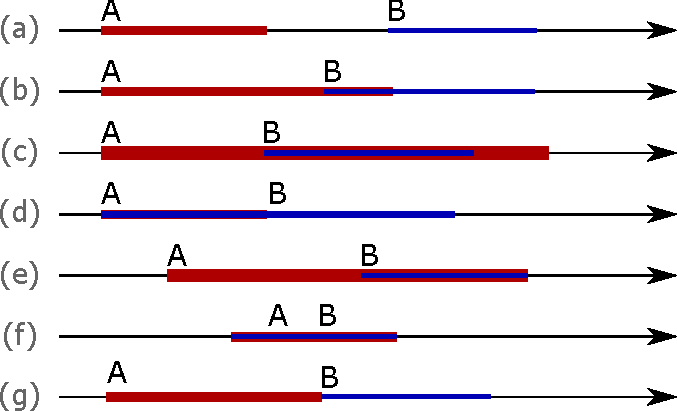
\includegraphics[width=0.6\textwidth]{time-relations.pdf}
  \caption{Relation of two events with duration}
  \label{fig:time-relations}
\end{figure}

\section{Structure expressions}
\label{sec:structure-expressions}

Structure expressions in \ac{FTA} are defined in terms of set theory, using symbols for fault events occurrence.
%, using what is called of generative sets.
If a fault event symbol is in a set, then it means that that fault has occurred.
A set is a combination of fault events that causes the top-level event of a tree.
A structure expression of a tree is denoted by a set of sets of fault event combinations.
The OR gate becomes the union operator between sets and the AND gate, the intersection.
For example, if a system contains fault events \emph{a}, \emph{b}, and \emph{c}, fault trees for this system contain at most all these three events.
%The occurrence of a single event $a$ may be associated with the occurrence (or not) of the other events in any order.
The occurrence of the fault event $a$ is denoted by a set of sets $A$, which contains the following sets:
%
\begin{enumerate}
  \item\label{item:fta-only-a-occurs} $\left\{a\right\}$: only \emph{a} occurs;
  \item\label{item:fta-a-and-b-occur} $\left\{a,b\right\}$: \emph{a} and \emph{b} occur;
  \item\label{item:fta-a-and-c-occur} $\left\{a,c\right\}$: \emph{a} and \emph{c} occur;
  \item\label{item:fta-all-occur} $\left\{a,b,c\right\}$: all three events occur.
\end{enumerate}
%
%Fault event \emph{a} occurs in all possibilities.
%As these are sets, they represent combinations and not permutations.
%Combination $\left\{a,b,c\right\}$ represents the same as $\left\{b,a,c\right\}$, $\left\{c,b,a\right\}$, etc.
%Let the set that contains these sets be $A$.
%Similarly, let $B$ be the set of sets that contain the fault event $b$.

The fault tree in \cref{fig:ex-fault-tree1} contains only two events and the resulting structure expression for this tree is the expression $A \inter B$ ($TOP$), where $A$ and $B$ are the sets of sets that contain $a$ and $b$, respectively.
The resulting combinations for $TOP$ are $\left\{a,b\right\}$ and $\left\{a,b,c\right\}$ (fault events \emph{a} and \emph{b} occur in all possibilities).\todo{Pedir para Alexandre avaliar pontualmente esta frase}

\begin{figure}[t]
  \centering
  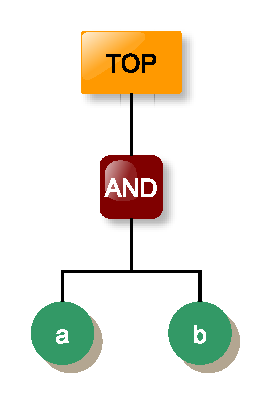
\includegraphics[width=0.3\textwidth]{ex-fault-tree1}
  \caption{Very simple example of a fault tree}
  \label{fig:ex-fault-tree1}
\end{figure}

After obtaining structure expressions, the next step is to reduce the expressions to a canonical form to obtain the \emph{minimal cut sets}.
Minimal cut sets are the sets that contain the minimum and sufficient events to activate the top-level failure.
That is, minimal cut sets are the smallest sets of fault event that, if all occur, cause the top-level failure to occur.
Probabilistic analysis is then performed on these events to obtain the overall probability of occurrence of the top-level event.
The \FThandbook shows an algorithm based on Shannon's method to reduce structure expressions to obtain minimal cut sets.
%BDDs are essentially the diagrams of Shannon's method.
The Boolean expression of the tree shown in \cref{fig:ex-fault-tree1} is $TOP = A \wedge B$.

Structure expressions are also present in \acp{TFT}~\cite{WP2009,Walker2009,WP2010}, through the \pandora methodology.
These expressions use the \ac{FTA} operators OR and AND, and three new operators related to events ordering: Priority-AND (PAND), Priority-OR (POR), and Simultaneous-AND (SAND).
The semantics of the PAND in \acp{TFT} is similar to the semantics of the Priority-AND described in the \FThandbook.
To avoid ambiguous expressions, the semantics in \acp{TFT} is stated in terms of natural numbers, using a \emph{sequence value} function.
For every possibility it assigns a sequence value to each fault event.
For example, if event A occurs before event B, then the sequence value of A is lower than the sequence value of B, and one formula to express this is A PAND B.

An invariant on sequence values is that there are no gaps for assigned values higher than zero.
For example, if faults A and B occur at the same time and there are only these two events, then they should both be assigned value $1$.
On the other hand, if A occurs before B, then the assigned values are 1 and 2, respectively.
Value zero means that the event is not active on the combination.
\Cref{tbl:tft-operators} shows the semantics of all \ac{TFT} operators.

\begin{table}
% table caption is above the table
\caption{\ac{TFT} operators and sequence value numbers}
\label{tbl:tft-operators}
% For LaTeX tables use
\begin{tabular}{ccccccc}
\hline\noalign{\smallskip}
A & B & AND & OR & PAND & POR & SAND  \\
\noalign{\smallskip}\hline\noalign{\smallskip}
0 & 0 & 0 & 0 & 0 & 0 & 0\\
0 & 1 & 0 & 1 & 0 & 0 & 0\\
1 & 0 & 0 & 1 & 0 & 1 & 0\\
1 & 1 & 1 & 1 & 0 & 0 & 1\\
1 & 2 & 2 & 1 & 2 & 1 & 0\\
2 & 1 & 2 & 1 & 0 & 0 & 0\\
\noalign{\smallskip}\hline
\end{tabular}
\end{table}

The reduction of \ac{TFT} expressions is achieved using dependency trees.
In a dependency tree, if all children of a tree node are true, then the node is also true.
Conversely, if a node is true, then all its children are also true.
An issue with dependency trees is that they grow exponentially.
Accordingly to the work reported in~\cite{WP2010}, it is already infeasible to deal with seven fault events in TFTs.
They use an alternative solution based on modularisation and algebraic laws~\cite{WP2009} to tackle this.

Structure expressions are also used in \acp{DFT}.
In~\cite{Merle2010,MRL+2010,MRL2011} fault events occur in a specific time and are instantaneous (similar to detected faults), stated through a ``date-of-occurrence'' function.
As the ``date-of-occurrence'' function is stated in continuous time, the probability of two events occurring at the same time is negligible.
In fact, useful information is obtained from the possibilities of relation in time of the occurrence of the events.

The work reported in~\cite{Merle2010,MRL+2010,MRL2011} describe an algebra with operators OR and AND, and three new operators to express events ordering: (i) non-inclusive-before, (ii) simultaneous, and (iii) inclusive-before.
The non-inclusive-before and the simultaneous operators are similar to \ac{TFT}'s POR and SAND operators, respectively.
The inclusive-before is a composition of the non-inclusive-before and the simultaneous operators.

The work reported in~\cite{TXD2011,XTD2012} shows the top-level events probability calculation for \acp{DFT} by converting them to a simplified version, using only order-based operators.
Such a simplified version, which is based on a modified \ac{BDD} that includes an order-based operator, creates Sequential BDDs that are used to perform the probabilistic analysis.

From the previous explanation, we can conclude that there is an omnipresence of order-based operators to analyse \acp{TFT} and \acp{DFT}.
And that each approach describes a new algebra based on different representations of events ordering with similar theorems to reduce expressions to a canonical form.

\section{Systems' nominal model and faults injection}
\label{sec:faults-injection}

Control system modelling using \simulink block diagrams~\cite{MathWorks2010} is recommended in~\cite{Nise1992} and have been used by our industrial partner.
%We follow this recommendation in this work.
It is a complementary tool of \matlab~\cite{MathWorks2010c}.
% ## TODO: melhorar essa frase
In fact, it works as a graphical interface to \matlab.
A \simulink model has blocks and connections between these blocks, named signals.
Each block has inputs and outputs and an internal behaviour expressed by its mathematical formula, which defines a function of the inputs for each output.
There are many predefined blocks in the tool.
It is also possible to create new blocks or use subsystems that encapsulate other blocks.
A simulation adds extra parameters to a block diagram, like elapsed time and time between states.
The elapsed time of a simulation is an abstraction for the quantity of possible simulation states and the time between states is related to the lowest common denominator of the sample time.
Some components define different sample times, depending on their mode of operation.
Usually, the value for this property is set to \textsim{auto}, allowing \simulink to choose a proper value automatically.

% \begin{figure*}[!t] \centering
%     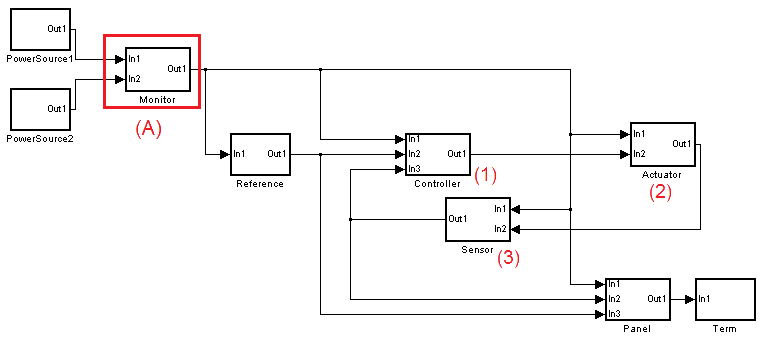
\includegraphics[width=0.8\linewidth]{acsBlockDiagrams}
%     \caption{\textpt{Diagrama em blocos do ACS fornecido pela
%     \EMBRAER.}\texten{Block diagram of the ACS provided by \EMBRAER}}
%     \label{fg:acsBlockDiagrams}
% \end{figure*}
\begin{figure}[t] \centering
  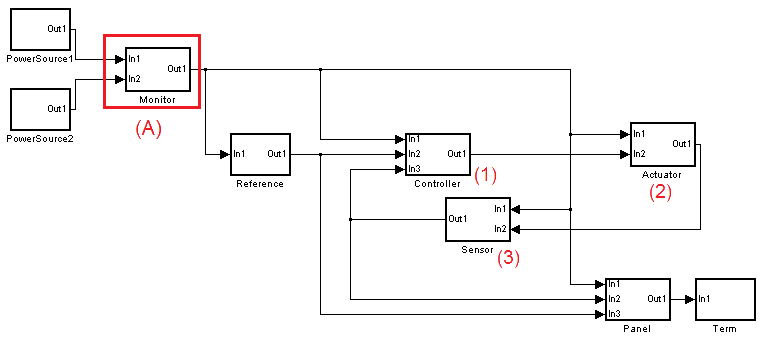
\includegraphics[width=\textwidth]{acsBlockDiagrams}
  \caption{Block diagram of the ACS provided by \EMBRAER (nominal model)}
  \label{fg:acsBlockDiagrams}
\end{figure}

Nowadays, control systems are usually composed of an electromechanical part and a processor.
\Cref{fg:acsBlockDiagrams} shows the components of a feedback system~\cite{AM2008} which was provided by \EMBRAER.
In this system, the feedback behaviour is given by the \textsim{Controller} (1), \textsim{Actuator} (2) and \textsim{Sensor} (3). A command is received by the \textsim{Controller}, which sends a signal to the \textsim{Actuator} to start its movement.
The \textsim{Sensor} detects the actual position of the \textsim{Actuator} and sends it back to the \textsim{Controller}, which adjusts the given command to achieve the desired position. This loop (feedback) continues until the desired position given by the original command is reached.

\begin{figure}[t] \centering
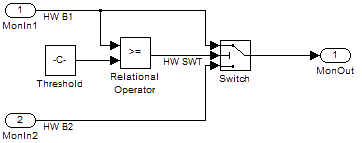
\includegraphics[width=0.6\textwidth]{blockDiagramMonitorInternals}
  \caption{Internal diagram of the monitor component (\cref{fg:acsBlockDiagrams}~(A)).}
  \label{fg:blockDiagramMonitorInternals}
\end{figure}

\Cref{fg:blockDiagramMonitorInternals} shows the internal elements of the monitor component (\cref{fg:acsBlockDiagrams}~(A)), which is used as case study in \cref{sec:case-study} to illustrate our
strategy.
The outputs of the hardware elements are annotated with \textsim{HW}, which are the two power sources and an internal component of the monitor (switch command).

\todo{Verificar se as frases tiradas da introdução se adequam melhor aqui.}
%As hardware components are susceptible to fault injection, this strategy consists of: (i) a process that represents the nominal behaviour (without fault injection), (ii) a process that represents the erroneous behaviour with all possibilities of faults, due to fault injection, and (iii) an observer process to compare the nominal behaviour with the erroneous behaviour.
%To create failure logic, we abstract the fault traces by not considering events ordering.




To perform a formal verification in a \simulink system design model, the work reported in~\cite{JMS+2011} translates a \simulink model to the \ac{cspm} language.
%
The resulting \ac{cspm} code is then used to check if it meets functional requirements also encoded in \ac{cspm
}.

In our previous work, reported in~\cite{DM2012}, we modified such a translation to perform fault injection using hardware annotations allowing a subsystem or part to ``break'' randomly.
%
We designed a \ac{cspm} process to act as an observer, watching outputs of the nominal version and comparing to the outputs of the ``breakable'' version (with injected faults) of the system.
%
When the \ac{cspm} process of the model and the observer are loaded into the \acs{fdr} model-checker, counter-examples are generated for each output that differs from the nominal model, thus obtaining a \emph{sequence} of injected faults combinations that leads to the unexpected output, which are indeed \emph{fault traces}.

In what follows, injected faults and the top-level failure have generic names based on the names of the \simulink model blocks.
It is out of the scope of~\cite{DM2012} to define event names.

For the \simulink model shown in~\cref{fg:blockDiagramMonitorInternals}, some representative fault traces are:

\begin{snippetcspm}[1]
TRACE 1:
failure.Hardware.N04_RelationalOperator.1.EXP.B.true
failure.Hardware.N04_RelationalOperator.1.ACT.B.false
failure.Hardware.N04_MonIn2.1.EXP.I.5
failure.Hardware.N04_MonIn2.1.ACT.OMISSION
out.1.OMISSION

TRACE 2:
failure.Hardware.N04_MonIn2.1.EXP.I.5
failure.Hardware.N04_MonIn2.1.ACT.OMISSION
failure.Hardware.N04_RelationalOperator.1.EXP.B.true
failure.Hardware.N04_RelationalOperator.1.ACT.B.false
out.1.OMISSION

TRACE 3:
failure.Hardware.N04_MonIn1.1.EXP.I.5
failure.Hardware.N04_MonIn1.1.ACT.OMISSION
failure.Hardware.N04_MonIn2.1.EXP.I.5
failure.Hardware.N04_MonIn2.1.ACT.OMISSION
out.1.OMISSION

TRACE 4:
failure.Hardware.N04_MonIn2.1.EXP.I.5
failure.Hardware.N04_MonIn2.1.ACT.OMISSION
failure.Hardware.N04_MonIn1.1.EXP.I.5
failure.Hardware.N04_MonIn1.1.ACT.OMISSION
out.1.OMISSION

TRACE 5:
failure.Hardware.N04_MonIn1.1.EXP.I.5
failure.Hardware.N04_MonIn1.1.ACT.OMISSION
failure.Hardware.N04_RelationalOperator.1.EXP.B.false
failure.Hardware.N04_RelationalOperator.1.ACT.B.true
out.1.OMISSION

TRACE 6:
failure.Hardware.N04_MonIn1.1.EXP.I.5
failure.Hardware.N04_MonIn1.1.ACT.OMISSION
failure.Hardware.N04_RelationalOperator.1.EXP.B.false
failure.Hardware.N04_RelationalOperator.1.ACT.B.true
failure.Hardware.N04_MonIn2.1.EXP.I.5
failure.Hardware.N04_MonIn2.1.ACT.OMISSION
out.1.OMISSION

TRACE 7:
failure.Hardware.N04_MonIn1.1.EXP.I.5
failure.Hardware.N04_MonIn1.1.ACT.OMISSION
failure.Hardware.N04_MonIn2.1.EXP.I.5
failure.Hardware.N04_MonIn2.1.ACT.OMISSION
failure.Hardware.N04_RelationalOperator.1.EXP.B.false
failure.Hardware.N04_RelationalOperator.1.ACT.B.true

TRACE 8:
failure.Hardware.N04_MonIn2.1.EXP.I.5
failure.Hardware.N04_MonIn2.1.ACT.OMISSION
failure.Hardware.N04_MonIn1.1.EXP.I.5
failure.Hardware.N04_MonIn1.1.ACT.OMISSION
failure.Hardware.N04_RelationalOperator.1.EXP.B.false
failure.Hardware.N04_RelationalOperator.1.ACT.B.true
\end{snippetcspm}
%
where \verb$N04$ is the subsystem name of the monitor in the \simulink diagram, \verb$MonIn1$ (first input of the monitor), \verb$MonIn2$ (second input of the monitor), and \verb$RelationalOperator$ (switcher controller) are the names of the hardware components in the \simulink diagram.

We only show eight counter-examples, but FDR generates a total of 64 counter-examples for this system.
The other counter-examples are similar to the traces shown with different internal events.

To reuse \hiphops, which is based on \acp{SFT}, each fault trace is abstracted as a conjunction (AND combination of the inner events), and the several conjunction-based fault events are combined using ORs (disjunctions).
%
The result of the combination is a Boolean expression that represents the conditions that cause an undesirable output, the failure logic of the model.

If the failure logic is obtained for a whole system, it is indeed the structure expression of a fault tree for a general failure as the top-level event.
Although it is possible to obtain the failure logic for a larger system, it may be impractical due to state-space explosion in \ac{cspm} model analysis.
Thus it should be used for components and subsystems or small systems following \hiphops compositional structure.
%
%Failure logic is used as the input of the strategy presented in~\cite{MJG+2010}.
Using failure logic as subsystem annotations in~\cite{PMS+2001}, it is possible to obtain structure expressions for a larger system.
It is worth noting that the goal of the work reported in~\cite{DM2012} was to connect with \hiphops, which is based on static fault trees.
But we already knew that we had a richer fault modelling information than that presented in~\cite{DM2012} because we abstracted traces (which already capture fault events ordering) to create propositions (any fault events order combination).
%In the works reported in~\cite{APR+2013,AFP+2013,AIP+2014}, fault modelling was used to verify if a system model is fault tolerant with respect to undesirable critical failures.
%The faults were explicitly modelled, and the analysis starts after the preliminary analysis of faults.
%Instead of modelling faults directly in a model, it is possible to inject faults without explicit fault modelling.
%This allows the system to break in hardware parts.

%Each injected fault appears on the trace as two events: the expected (\verb$EXP$) value of the nominal system and the actual (\verb$ACT$) value used on the breakable system.
%For example, in \verb$TRACE 1$, the expected output of the switcher (\verb$N04_RelationalOperator$) is true, but the actual value is false.

To show how these traces become failure logic, let us abbreviate fault names as:
%
\begin{snippetcspm}[2]
A = failure.Hardware.N04_MonIn1.1
B = failure.Hardware.N04_MonIn2.1
S = failure.Hardware.N04_RelationalOperator
\end{snippetcspm}
%
So, for each trace, we obtain an expression:
\begin{align*}
\mathtt{TRACE\,1} &= S \land B\\
\mathtt{TRACE\,2} &= B \land S\\
\mathtt{TRACE\,3} &= A \land B\\
\mathtt{TRACE\,4} &= B \land A\\
\mathtt{TRACE\,5} &= A \land S\\
\mathtt{TRACE\,6} &= A \land S \land B\\
\mathtt{TRACE\,7} &= A \land B \land S\\
\mathtt{TRACE\,8} &= B \land A \land S
\end{align*}

And we combine them as a single Boolean expression:
%
$\mathtt{TRACE\,1} \lor \mathtt{TRACE\,2} \lor \mathtt{TRACE\,3} \lor \mathtt{TRACE\,4} \lor \mathtt{TRACE\,5} \lor \mathtt{TRACE\,6} \lor \mathtt{TRACE\,7} \lor \mathtt{TRACE\,8}$, %
which by a traditional boolean reduction strategy results in:
%
\[(A \land B) \lor (S \land (A \lor B))\]

\begin{sloppypar}
The above expression is exactly the same failure logic expression provided by \EMBRAER if we use the following association (\cref{tbl:acsAnnotations}):
\begin{align*}
A &= \text{LowPower-In1}\\
B &= \text{LowPower-In2}\\
S &= \text{SwitchFailure}
\end{align*}
\end{sloppypar}

\begin{table}[t]
\renewcommand{\arraystretch}{1.3}
\caption{Annotations table of the ACS provided by \EMBRAER}
\label{tbl:acsAnnotations}
\centering
\begin{tabularx}{\linewidth}{|c|c|c|X|}
\hline
\bfseries Component & \bfseries Deviation & \bfseries Port & \bfseries Annotation \\
\hline
PowerSource & LowPower & Out1 & PowerSourceFailure\\
\hline
Monitor & LowPower & Out1 & (SwitchFailure AND (LowPower-In1 OR LowPower-In2)) OR (LowPower-In1 AND LowPower-In2) \\
\hline
Reference & OmissionSignal & Out1 & ReferenceDeviceFailure OR LowPower-In1\\
\hline
\end{tabularx}
\end{table}

Note that when we combine each fault with ANDs, we lose the information about order\footnote{In our previous work we designed the observer to ignore order as well, by making similar traces---with different ordering---the same size. Here we modified the observer specification to make similar traces with different sizes.}: $S \land B$ and $B \land S$ are equal, due to the commutative law of Boolean expressions.

Our strategy finds fault combinations $S$ and $B$ (in the sense of $S$ occurring before $B$) as well as $B$ and $S$ (in the sense of $B$ occurring before $S$) but abstracts this ordering information obtaining $B$ and $S$, which is equivalent to $S$ and $B$ in Boolean Algebra.
%
If $A$ fails before $S$, the system fails because it should switch to $B$, but the switcher is in a faulty state.
%
On the other hand, if $S$ fails before $A$, the switcher fails because it inadvertently switched to $B$ when $A$ was still operational.
%
When $A$ fails, nothing changes and the output of the system is obtained from $B$.

We also employed the strategy proposed in the work~\cite{DM2012} in another case study and obtained a weaker failure expression (that is, our expression considers more cases).
The failure expression provided by the engineers of our industrial partner was stronger because they considered that one component has a very low probability of failure and removed it from the failure analysis.
Although acceptable, it may cause incorrect analysis.
Our strategy avoids this kind of issue by being completely systematic.


\chapter{A free algebra to express structure expressions of ordered events}
\label{sec:strategy}

Recall from \cref{sec:time-relations,sec:structure-expressions} that fault events are independent on one another if the events are not susceptible to a common cause.
The set-theoretical abstraction of structure expressions for \acp{SFT}~\cite[pp. VI-11]{VGR+1981} is very close to \iac{fba}, where each generator in \acp{fba} corresponds to a fault event symbol in fault trees.
In \acp{fba}, as generators are ``free'', they are independent on one another and Boolean formulas are written as a set of sets of possibilities, which are similar to the structure expressions of \acp{SFT}.
%This is equivalent to the disjunctive normal form, where each set is a minterm (conjunction) and the formula itself is the disjunction of minterms.

The set of sets for \acp{fba} are the denotational semantics for Boolean algebras.
We use the concept of generators to define the denotational semantics of \ac{algebra} using a set of lists without repetition (distinct lists).
The choice of lists is because this structure inherently associates a generator to an index, making implicit the representation of order.
These lists are composed by non-repeated elements (distinct lists) because the events in fault trees are non-repairable, thus they do not occur more than once.

This list representation is different from the Sequence Number function used in~\cite{WP2009,Walker2009}, but is related to the concept that there should be no gaps between consecutive events occurrence.
It is different because order 0 (zero) in~\cite{WP2009,Walker2009} means non-occurrence.
It may cause a discontinuity because 0 to 1 is different of 1 to 2.
In \acp{fba} the non-occurrence of an event is just the absence of the event, thus we use the same representation of non-occurrence in \ac{algebra} to avoid this discontinuity.

%The work reported in~\cite{MRL2011,Merle2010} uses continuous time and the relations of events is obtained from a ``date-of-occurrence'' function.
%It is related to the detection of an event as discussed in~\cref{sec:time-relations,sec:structure-expressions} and the useful information is in fact the order of occurrence of the events, not the date-of-occurrence itself.


%In our previous work, we used this technique of using fault injection to reuse a nominal model without explicit fault modelling, obtaining Boolean expressions of systems' failures, as we showed in \cref{sec:faults-injection}.
%The drawback of this approach is that fault events ordering information is lost because it is not relevant on the Boolean expressions extraction.

From the need to tackle events ordering and from the ordering information we had from fault injection that we developed in~\cite{DM2012}, we defined a lists-based algebra, called \ac{algebra}, to express and analyse systems considering events ordering.
We also provide a mapping from fault traces~\cite{DM2012} (from \ac{cspm} models) to this algebra.
The order-specific operations are expressed with a new operator ($\xbeforeop$) that we call XBefore (or exclusive before).

%We show reduction laws relating the XBefore operator to traditional Boolean operators.
%It is important to note that we support a NOT operator in our algebra.

%\usepackage{graphics} is needed for \includegraphics
%\begin{figure}[t]
%\begin{center}
  %\includegraphics[width=0.5\textwidth]{strategy}
%  \caption{Strategy overview}
%  \label{fig:overview}
%\end{center}
%\end{figure}

%It is defined as a set of all sets of distinct lists, called $\algebraset$.
%Then we show that all Boolean operators takes elements from and into $\algebraset$.

%We now show the \ac{algebra} as a set of all possible formulas.
In the following we show the definitions and laws of our proposed \ac{algebra}.
To avoid repetition, let $S$, $T$ and $U$ be sets of distinct lists.
A list $xs$ is distinct if it has no repeated element.
So, if $x$ is in $xs$, then it has a unique associated index $i$ and we denote it as $x = \nth{xs}{i}$.
Furthermore, as we follow \iac{fba} characterisation, we also need to show that the generators are independent.

The \ac{algebra} form a free algebra, similarly to \acp{fba}.
\emph{Infimum} and \emph{Supremum} are defined as set intersection ($\inter$) and union ($\union$) respectively.
The order within the algebra is defined with set inclusion ($\subseteq$).

To distinguish the permutations that are not defined in \ac{fba}, we need a new operator.
We give the definition of XBefore ($\xbeforeop$) in terms of list concatenation, similar to the work reported in~\cite{DM2015}:
%
\begin{equation}
\label{def:xbefore-append}
\xbefore{S}{T} =
  \setsin{
    zs | \exists xs, ys \bullet \parsin{\listset{xs}} \inter \parsin{\listset{ys}} = \{\}
      \land xs \in S \land ys \in T \land zs = \append{xs}{ys}
  }
\end{equation}
%
where the $\listset{}$ function returns the set of the elements of a list, and $\append{}{}$ concatenates two lists.

In some cases it is more intuitive to use the XBefore definition in terms of lists slicing because it uses indexes explicitly.
%\Cref{thm:xbefore} shows that the two definitions are equivalent.
Lists slicing is the operation of taking or dropping elements, obtaining a sublist.
In slicing, the starting index is inclusive, and the ending is exclusive.
Thus the first index is 0 and the last index is the list length.
For example, the list $\slice{xs}{i}{\length{xs}}$ is equal to the $xs$ list, where $\length{xs}$ is the list length.
We use the following notation for list slicing:
%
\begin{subequations}
\begin{align}
\slice{xs}{i}{j} &= \text{starts at $i$ and ends at $j-1$}\\
\sliceright{xs}{j} &= \slice{xs}{0}{j}\\
\sliceleft{xs}{i} &= \slice{xs}{i}{\length{xs}}
\end{align}
\end{subequations}

List slicing and concatenation are complementary: concatenating two consecutive slices results in the original list:
\begin{equation}
\forall i \bullet \append{\sliceright{xs}{i}}{\sliceleft{xs}{i}} = xs
\end{equation}

There is an equivalent definition of XBefore with concatenation using lists slicing:
%
\begin{equation}
\xbefore{S}{T} =
  \setsin{
    zs | \exists i \bullet \sliceright{zs}{i} \in S \land \sliceleft{zs}{i} \in T
  }
\end{equation}

A variable in \ac{algebra} is defined by one generator, and denotes its occurrence:
%
\begin{equation}
\label{def:var}
\var{x} =
  \setsin{
    zs | x \in zs
  }
\end{equation}

The following expressions are sufficient to define the \ac{algebra} in terms of an inductively defined set ($\algebraset$):
%
\begin{subequations}
\label{def:algebraset}
\begin{align}
\var x & \in \ac{algebra}set & \text{Variable}\label{def:algebraset-var}\\
S \in \algebraset \implies -S & \in \algebraset & \text{Complement, Negation}\label{def:algebraset-compl}\\
S \in \algebraset \land T \in \algebraset \implies S \inter T & \in \algebraset & \text{Intersection, \emph{Infimum}}\label{def:algebraset-inf}\\
S \in \algebraset \land T \in \algebraset \implies \xbefore{S}{T} & \in \algebraset & \text{XBefore}\label{def:algebraset-xbefore}\\
\intertext{Following the definitions, the expressions below are also valid for $\algebraset$:}
\True &\in \algebraset & \text{Universal set, True}\label{def:algebraset-true}\\
\False &\in \algebraset & \text{Empty set, False}\label{def:algebraset-false}\\
S \in \algebraset \land T \in \algebraset \implies S \union T &\in \algebraset & \text{Union, \emph{Supremum}}\label{def:algebraset-sup}
\end{align}
\end{subequations}

The following expressions are valid for generators $a$ and $b$ and are sufficient to show that the generators are independent:
%
\begin{subequations}
\label{eqs:generators-independence}
\begin{align}
&\var a \subseteq \var b \iff a = b\label{eqs:generators-independence-subseteq-eq}\\
&\var a = \var b \iff a = b\\
&\var a \not\subseteq - \var b\\
&\var a \neq -\var b\label{eqs:generators-independence-subseteq-neq-compl} \\
&- \var a \not\subseteq \var b\\
&- \var a \neq \var b\label{eqs:generators-independence-subseteq-compl-neq}
\end{align}
\end{subequations}

Expressions \eqref{def:algebraset-var} to \eqref{def:algebraset-sup} and \eqref{eqs:generators-independence-subseteq-eq} to \eqref{eqs:generators-independence-subseteq-compl-neq} implies that the \ac{algebra} without the XBefore operator \eqref{def:xbefore-append} forms a Boolean algebra based on sets of lists.
And this is also equivalent to \iac{fba} with the same generators.

In our previous work~\cite{DM2015} we stated a relation of XBefore and \emph{supremum}, provided the operands are variables \eqref{def:var}.
Now we generalise this relation in terms of abstract properties of the operands of the XBefore.
We name these properties as \emph{temporal properties}.
%and show them in \cref{sec:temporal-properties}.

\section{Temporal properties (\emph{\tempotext})}
\label{sec:temporal-properties}

Temporal properties give a more abstract and less restrictive shape\todo{touch?} on the XBefore laws.
These properties avoid the requirement that every operand of XBefore should be a variable \eqref{def:var}.
%The properties are: $\tempo[1]{}$ (\cref{def:tempo1}), $\tempo[2]{}$ (\cref{def:tempo2}), $\tempo[3]{}$ (\cref{def:tempo3}), and $\tempo[4]{}$ (\cref{def:tempo4}).

The first temporal property is about disjoint split.
If the first part of a list is in a given set, then every remainder part is not.
So, if a generator is in the beginning of a list, it must not be at the ending (and vice-versa).
%
%\todo{Explain temporal properties with respect to Figure 1 about relation of events? At least make it clearer.}
%
\begin{subequations}
\begin{align}
\tempo[1]{S} &= \forall i, j, zs \bullet
  i \le j \implies
  \lnot \left(
    \sliceright{zs}{i} \in S \land \sliceleft{zs}{j} \in S
  \right)\label{def:tempo1}\\
\tempo[2]{S} &= \forall i, zs \bullet
  zs \in S \iff
  \sliceright{zs}{i} \in S \lor \sliceleft{zs}{i} \in S\label{def:tempo2}\\
\tempo[3]{S} &= \forall i, j, zs \bullet
  j < i \implies
  \left(
    \slice{zs}{j}{i} \in S \iff \sliceright{zs}{i} \in S \land \sliceleft{zs}{j} \in S
  \right)\label{def:tempo3}\\
\tempo[4]{S} &= \forall zs \bullet zs \in S \iff (\exists i \bullet \slice{zs}{i}{\left(i+1\right)} \in S)\label{def:tempo4}
%\intertext{Replace $\tempo[4]{S}$ by (less restrictive):}
%&= \forall zs \bullet zs \in S \iff \exists i,j \bullet i < j \land \slice{zs}{i}{j} \in S
\end{align}
\end{subequations}

The second temporal property is about belonging to one sublist in the beginning or in the end.
If a generator is in a list, then it must be at the beginning or at the ending.
%
%\begin{definition}[\Tempotext 2, belongs to one sublist in the beginning or at the ending]
%\label{def:tempo2}
%Let $S$ be a set of distinct lists:
%\end{definition}
%

The third temporal property is about belonging to one sublist in the middle.
If a generator belongs to a sublist between $i$ and $j$, then it belongs to the sublist that starts at first position and ends in $j$ and to the sublist that starts at $i$ and ends at the last position (both sublists contain the sublist in the middle).
%
%\begin{definition}[\Tempotext 3, belongs to the middle of a sublist]
%\label{def:tempo3}
%Let $S$ be a set of distinct lists:
%\end{definition}
%

Finally, if a generator belongs to a list, then there is a sublist of size one that contains the generator.
%
%\begin{definition}[\Tempotext 4, belongs to one sublist of size one]
%\label{def:tempo4}
%Let $S$ be a set of distinct lists:
%\end{definition}
%

Variables have all four temporal properties. For a generator $x$, the following is valid:
%
\[
\tempo[1]{\left(\var{x}\right)} \land
\tempo[2]{\left(\var{x}\right)} \land
\tempo[3]{\left(\var{x}\right)} \land
\tempo[4]{\left(\var{x}\right)}
\]

\begin{sloppypar}
In our previous work~\cite{DM2015} we used set difference to specify the XBefore operator.
Provided $\tempo[1]{S}$ and $\tempo[1]{T}$, XBefore in~\cite{DM2015} is equivalent to \eqref{def:xbefore-append}:
%
\begin{equation}
\xbefore{S}{T} = \left\{ zs | \exists xs, ys \bullet xs \in S-T \land ys \in T-S \land \distinct{zs} \land zs = \append{xs}{ys}  \right\}
\end{equation}
\end{sloppypar}

Other expressions also meet one or more temporal properties:
\begin{subequations}
\begin{align}
\tempo[1]{S} \land \tempo[1]{T} & \implies \tempo[1]{\parsin{S \inter T}}\\
\tempo[3]{S} \land \tempo[3]{T} & \implies \tempo[3]{\parsin{S \inter T}}\\
\tempo[2]{S} \land \tempo[2]{T} & \implies \tempo[2]{\parsin{S \union T}}\\
\tempo[4]{S} \land \tempo[4]{T} & \implies \tempo[4]{\parsin{S \union T}}
\end{align}
\end{subequations}

\section{XBefore laws}
\label{sec:xbefore-laws}

We now show some laws to be used in the algebraic reduction of \ac{algebra} formulas.
The laws follow from the definition of XBefore, from events independence, and from the temporal properties.

We use a normal form similar to the disjunctive normal form (DNF) of Boolean algebra.
In DNF each sub-expression is a minimal cut set for \ac{SFT}.
In our normal form, also called DNF, we allow ANDs, NOTs, and XBefores to be in the sub-expressions.
Each sub-expression is a set of minimal cut sequences for \ac{TFT} and \ac{DFT}.
The following formulas are in DNF:
%
\begin{align*}
&\parsin{A \inter -B} \union \parsin{\parsin{\xbefore{A}{B}} \inter C}\\
&A \union B\\
&\xbefore{A}{B}\\
&A \inter B\\
&\xbefore{\xbefore{A}{B}}{C}
\end{align*}
%
The following formulas are \emph{not} in DNF:
%
\begin{align*}
&-\parsin{A \union B}\\
&A \inter \parsin{B \union C}\\
&\xbefore{A}{\parsin{B \union C}}\\
&\xbefore{A}{\parsin{B \inter C}}
\end{align*}

But to transform the last two formulas into DNF, one can use Laws \eqref{thm:xbefore-sup-1},~\eqref{thm:xbefore-sup-2},~\eqref{thm:xbefore-inf-1} and~\eqref{thm:xbefore-inf-2}, for instance.

We define events independence ($\independenteventsop$) as the property that one operand does not imply the other.
For example, we need to avoid that the operands of XBefore are $\var{a}$ and $\var{a} \union \var{b}$ (it results in $\False$, see \eqref{thm:xbefore-not-idempotent}).
%
\begin{equation}
\independentevents{S}{T} = \forall i, zs \bullet
  \lnot \left(
    \slice{zs}{i}{\left(i+1\right)} \in S \land
    \slice{zs}{i}{\left(i+1\right)} \in T
  \right)
\end{equation}

The absence of occurrences ($\False$, the empty set of $\algebraset$) is a ``0'' for the XBefore operator.
%
\begin{subequations}
\begin{align}
\xbefore{\False}{S} =&
  \False &
  \text{left-false-absorb}
  \label{thm:xbefore-of-false-1}\\
%
\xbefore{S}{\False} =&
  \False &
  \text{right-false-absorb}
  \label{thm:xbefore-of-false-2}\\
%
\left(\xbefore{S}{T}\right) \union S =& S &
  \text{left-union-absorb}
  \label{thm:xbefore-sup-absorb-1}\\
%
\left(\xbefore{T}{S}\right) \union S =& S &
  \text{right-union-absorb}
  \label{thm:xbefore-sup-absorb-2}\\
%
\tempo[1]{S} \implies
  \xbefore{S}{S} =&
  \False &
  \text{non-idempotent}
  \label{thm:xbefore-not-idempotent}\\
%
\tempo[1]{S}\land\tempo[1]{T}\land \tempo[1]{U}\implies&\nonumber\\
  \xbefore{S}{(\xbefore{T}{U})} =&
  \xbefore{(\xbefore{S}{T})}{U} &
  \text{associativity}
%
\end{align}
\end{subequations}
%
The XBefore is absorbed by one of the operands: if one of the operands may happen alone, thus the order with any other operand is irrelevant.
However, an event cannot come before itself, thus XBefore is not idempotent.
The XBefore but is associative.

To allow formula reduction we need the relation of XBefore to the other Boolean operators.
First we use the XBefore as operands of union and intersection.
%
\begin{subequations}
\begin{align}
\tempo[1]{S} \land \tempo[1]{T}\implies&\nonumber\\
  \parsin{\xbefore{S}{T}} \inter \parsin{\xbefore{T}{S}} =&
  \False &
  \text{inter-equiv-false}
  \label{thm:xbefore-inf-equiv-bot}\\
%
\tempo{S} \land \tempo{T} \land \independentevents{S}{T}\implies&\nonumber\\
  \parsin{\xbefore{S}{T}} \union \parsin{\xbefore{T}{S}} =&
  S \inter T &
  \text{union-equiv-inter}
  \label{thm:xbefore-sup-equiv-inf}
%
\end{align}
\end{subequations}
%
As the XBefore is not symmetric, the intersection of symmetrical sets is empty.
The union of the symmetric is a partition of the intersection of the operands.

In our previous work~\cite{DM2015}, we stated that $S$ and $T$ had to be variables.
For example, of the form $\var{s}$ and $\var{t}$.
Now, each law requires that the operands satisfy some of the temporal properties, avoiding using variables explicitly.
%So, as variables satisfy all temporal properties and by \eqref{thm:xbefore-sup-equiv-inf}, our theorem ``Exclusive before \emph{supremum}'' is still valid.

Boolean operators are used as operands of the XBefore in the following laws.
%
\begin{subequations}
\begin{align}
\xbefore{\left(S \union T\right)}{U} =&
  \parsin{\xbefore{S}{U}} \union \parsin{\xbefore{T}{U}} &
  \text{left-union-dist}
  \label{thm:xbefore-sup-1}\\
%
\xbefore{S}{\left(T \union U\right)} =&
  \parsin{\xbefore{S}{T}} \union \parsin{\xbefore{S}{U}} &
  \text{right-union-dist}
  \label{thm:xbefore-sup-2}\\
%
\tempo{S} \land \tempo{T} \land \independentevents{S}{T} & \implies\nonumber \\
  \xbefore{\left(S \inter T\right)}{U} =&
  \parsin{\xbefore{\xbefore{S}{T}}{U}} \union \nonumber\\
  &\parsin{\xbefore{\xbefore{T}{S}}{U}} &
  \text{left-inter-dist}
  \label{thm:xbefore-inf-1}\\
%
\tempo{T} \land \tempo{U} \land \independentevents{T}{U} & \implies \nonumber\\
  \xbefore{S}{\left(T \inter U\right)} =&
  \parsin{\xbefore{S}{\xbefore{T}{U}}} \union \nonumber\\
  &\parsin{\xbefore{S}{\xbefore{U}{T}}} &
  \text{right-inter-dist}
  \label{thm:xbefore-inf-2}\\
%
\tempo[2]{S} \implies S \inter \parsin{\xbefore{T}{U}} =&
  \parsin{\xbefore{\parsin{S \inter T}}{U}} \union \nonumber\\
  &\parsin{\xbefore{T}{\parsin{S \inter U}}} &
  \text{unordered}
  \label{thm:and_xbefore_equiv_or_xbefore}
\end{align}
\end{subequations}
%
XBefore is distributive over union.
On the other hand, the intersection is related to order.
Thus it is not distributive with XBefore.
Finally, the intersection of an event with an XBefore states that such an event can occur in any order within the events in the XBefore.

The law name, unordered, of \eqref{thm:and_xbefore_equiv_or_xbefore} is clearer if we expand \eqref{thm:and_xbefore_equiv_or_xbefore} with \eqref{thm:xbefore-inf-1} and ~\eqref{thm:xbefore-inf-2}:
%
%\begin{subequations}
\begin{align}
\tempo{S} \land \tempo{T} \land \nonumber\\
  \tempo{U} \land \independentevents{S}{T} \land \independentevents{S}{U} & \implies \nonumber\\
  S \inter \parsin{\xbefore{T}{U}} = &
  \parsin{\xbefore{\xbefore{S}{T}}{U}} \union \nonumber\\
  & \parsin{\xbefore{\xbefore{T}{S}}{U}} \union \nonumber\\
  & \parsin{\xbefore{\xbefore{T}{U}}{S}} &
  \text{expanded-unordered}
  \label{thm:and_xbefore_equiv_or_xbefore_expanded}
%\\
%
%\tempo[2]{S} \implies S \inter \parsin{\xbefore{S}{T}} =& \xbefore{S}{T} &
%  \text{left-inter-absorb}
%  \label{thm:xbefore-inf-absorb-1}\todo{Prove this in Isabelle}\\
%
%
%\tempo[2]{S} \implies S \inter \parsin{\xbefore{T}{S}} =& \xbefore{T}{S} &
%  \text{right-inter-absorb}
%  \label{thm:xbefore-inf-absorb-2}\todo{Prove this in Isabelle}
\end{align}
%\end{subequations}
%
%From \eqref{thm:xbefore-not-idempotent} and~\eqref{thm:and_xbefore_equiv_or_xbefore}, intersection and XBefore also have an absorption law.


\chapter{Case study}
\label{sec:case-study}

\EMBRAER provided us with the \simulink model of an Actuator Control System (depicted in \cref{fg:acsBlockDiagrams}).
The failure logic of this system (that is, for each of its constituent components) was also provided by \EMBRAER (we show some of them in \cref{tbl:acsAnnotations}).
In what follows we illustrate our strategy using the Monitor component.

A monitor component is a system commonly used for fault tolerance~\cite{ONB2002,KK2007}.
Initially, the monitor connects the main input (power source on input port 1) with its output.
It observes the value of this input port and compares it to a threshold.
If the value is below the threshold, the monitor disconnects the output from the main input and connects to the secondary input.
We present the \simulink model for this monitor in \cref{fg:blockDiagramMonitorInternals}.

%As we mentioned in~\cref{sec:faults-injection} we translated the monitor to \ac{cspm} according to our strategy and modified the observer to make FDR generate more counter-examples.

Now we show two contributions: (i) using only Boolean operators, thus ignoring ordering, we can obtain the same results obtained in~\cite{DM2012}, and (ii) we represent each of the fault traces reported in~\cite{DM2012} as a term in our proposed algebra of temporal faults.
Similarly to the association of fault events of \cref{tbl:acsAnnotations} in \cref{sec:faults-injection}, we associate the fault events as:
%
\begin{align*}
a &= \text{LowPower-In1}& A = \var a\\
b &= \text{LowPower-In2}& B = \var b\\
s &= \text{SwitchFailure}& S = \var s
\end{align*}

\section{Structure expressions with Boolean operators}

In this section we show that the same result reported in~\cite{DM2012} in terms of static failure logic (or Boolean propositions) can be obtained with our boolean operator without using XBefore.
For each trace shown in \cref{sec:faults-injection}, a mapping function\footnote{In this work we do not show the mapping function from traces to \ac{algebra} (and the mapping function with XBefore in \cref{sec:case-study-xbefore}).
The mapping rules follow the traces: XBefore is obtained by the order of occurrence and the absence of an event is the complement ($-$).} ($\tracetobool$) generates the following sets of lists:
%
\begin{align*}
\text{\texttt{TRACE 1: }}&[s,b] \tracetobool S \inter B \inter -A & \setsin{\listsin{s,b},\listsin{b,s}}\\
\text{\texttt{TRACE 2: }}&[b,s] \tracetobool B \inter S \inter -A & \setsin{\listsin{s,b},\listsin{b,s}}\\
\text{\texttt{TRACE 3: }}&[a,b] \tracetobool A \inter B \inter -S & \setsin{\listsin{a,b},\listsin{b,a}}\\
\text{\texttt{TRACE 4: }}&[b,a] \tracetobool B \inter A \inter -S & \setsin{\listsin{a,b},\listsin{b,a}}\\
\text{\texttt{TRACE 5: }}&[a,s] \tracetobool A \inter S \inter -B & \setsin{\listsin{a,s},\listsin{s,a}}\\
\text{\texttt{TRACE 6: }}&[a,s,b] \tracetobool A \inter S \inter B & \setsin{\listsin{a,b,s},\listsin{a,s,b},\ldots,\listsin{s,b,a}}\\
\text{\texttt{TRACE 7: }}&[a,b,s] \tracetobool A \inter B \inter S & \setsin{\listsin{a,b,s},\listsin{a,s,b},\ldots,\listsin{s,b,a}}\\
\text{\texttt{TRACE 8: }}&[b,a,s] \tracetobool B \inter A \inter S & \setsin{\listsin{a,b,s},\listsin{a,s,b},\ldots,\listsin{s,b,a}}\\
\end{align*}

They represent the same faults shown in \cref{sec:faults-injection}.
Note that the negation in the formula is very simple to represent in \ac{algebra} (and \ac{fba}) because it is just the absence of the generator.

Combining the above sets with unions (ORs), we obtain the following formula set:
%
\[
\left\{ \listsin{s,b}, \listsin{b,s}, \listsin{a,b}, \listsin{b,a}, \listsin{a,s}, \listsin{s,a}, \listsin{a,b,s}, \listsin{a,s,b},\ldots,\listsin{s,b,a} \right\}
\]

If we use Boolean expression reduction instead, it results in the following expression in \ac{algebra} (and in \ac{fba}):
\[
(A \inter B) \union (S \inter (A \union B))
\]
%
which is equivalent to the set of sets above and is equivalent to \EMBRAER failure logic expression shown in \cref{tbl:acsAnnotations} (with ANDs as $\inter$ and ORs as $\union$).
%
This shows that \ac{algebra} can represent (static) failure logic as in our previous work~\cite{DM2012}.

\section{Structure expressions with XBefore}
\label{sec:case-study-xbefore}

Now, by using TFA with the XBefore operator and a mapping function ($\tracetoalgebra$), we can capture each possible individual sequences as generated by the work~\cite{DM2012}:
%
\begin{align*}
\text{\texttt{TRACE 1: }}&[s,b] \tracetoalgebra \parsin{\xbefore{S}{B}} \inter -A & \left\{[s,b]\right\}\\
\text{\texttt{TRACE 2: }}&[b,s] \tracetoalgebra \parsin{\xbefore{B}{S}} \inter -A & \left\{[b,s]\right\}\\
\text{\texttt{TRACE 3: }}&[a,b] \tracetoalgebra \parsin{\xbefore{A}{B}} \inter -S & \left\{[a,b]\right\}\\
\text{\texttt{TRACE 4: }}&[b,a] \tracetoalgebra \parsin{\xbefore{B}{A}} \inter -S & \left\{[b,a]\right\}\\
\text{\texttt{TRACE 5: }}&[a,s] \tracetoalgebra \parsin{\xbefore{A}{S}} \inter -B & \left\{[a,s]\right\}\\
\text{\texttt{TRACE 6: }}&[a,s,b] \tracetoalgebra \xbefore{\xbefore{A}{S}}{B} & \left\{[a,s,b]\right\}\\
\text{\texttt{TRACE 7: }}&[a,b,s] \tracetoalgebra \xbefore{\xbefore{A}{B}}{S} & \left\{[a,b,s]\right\}\\
\text{\texttt{TRACE 8: }}&[b,a,s] \tracetoalgebra \xbefore{\xbefore{B}{A}}{S} & \left\{[b,a,s]\right\}
\end{align*}

Using \ac{algebra} and combining each trace with ORs (unions), we obtain the following set:
%
\[
M_L =
  \left\{
    [a,b],[b,a],[b,s],[s,b],[a,s],
    [a,b,s],[a,s,b],[s,a,b]
  \right\}
\]

From the above traces, we also build \iac{algebra} expression by mapping each trace to an XBefore expression, composing all resulting XBefore expressions with ORs and reducing them using the XBefore laws (\cref{sec:xbefore-laws}), resulting in an expression ($M_A$) that is equivalent to the above set of lists ($M_L \equiv M_A$).
The failure expression of the monitor\footnote{In the final formula, $\parsin{B \inter S \inter -A} \union \parsin{A \inter B \inter -S}$ is equivalent to $\parsin{B \inter \parsin{S \oplus A}}$. There is a typo in our previous work \cite{DM2015}. The expression was written with an OR ($\lor$) but it should an XOR ($\oplus$).} is:
%
\begin{align*}
M_A = & \parsin{\parsin{\xbefore{S}{B}} \inter -A} \union \parsin{\parsin{\xbefore{B}{S}} \inter -A} \union\\
  &\parsin{\parsin{\xbefore{A}{B}} \inter -S} \union \parsin{\parsin{\xbefore{B}{A}} \inter -S} \union\\
  & \parsin{\parsin{\xbefore{A}{S}} \inter -B} \union \\
  & \parsin{\xbefore{\xbefore{A}{S}}{B}} \union \parsin{\xbefore{\xbefore{A}{B}}{S}} \union \parsin{\xbefore{\xbefore{B}{A}}{S}} \\
%%
= &\parsin{B \inter S \inter -A} \union & \text{by \eqref{thm:xbefore-sup-equiv-inf}}\\
  & \parsin{B \inter A \inter -S} \union & \text{by \eqref{thm:xbefore-sup-equiv-inf}}\\
  & \parsin{\parsin{\xbefore{A}{S}} \inter -B} \union\\
  & \parsin{\xbefore{\xbefore{A}{S}}{B}} \union \parsin{\xbefore{\xbefore{A}{B}}{S}} \union \parsin{\xbefore{\xbefore{B}{A}}{S}}\\
%
= &\parsin{B \inter S \inter -A} \union \\
  & \parsin{B \inter A \inter -S} \union \\
  & \parsin{\parsin{\xbefore{A}{S}} \inter -B} \union \\
  & \parsin{\parsin{\xbefore{A}{S}} \inter B} & \text{by \eqref{thm:and_xbefore_equiv_or_xbefore_expanded}}\\
%
= &\parsin{B \inter S \inter -A} \union \parsin{B \inter A \inter -S} \union \parsin{\xbefore{A}{S}} & \text{by absorption}
\end{align*}

The semantics of the above expression is: (i) fault $b$ ($\var{b}$) occurs and fault $a$ ($\var{a}$) or fault $s$ ($\var{s}$) occurs (but not both $a$ and $s$), or (ii) fault $a$ occurs before fault $s$, which is more precise than the expression found without considering order of events.

\section{Conclusion}
\label{sec:conclusion}

In this work we presented a foundational theory to support a more precise representation of fault events as compared to our previous strategy for injecting faults~\cite{DM2012}.
%
The failure logic is essential for system safety assessment because it is used as basic input for building fault trees~\cite{PMS+2001,JMS+2011,GMS+2010}.
%
%We use \simulink as starting point because it is a standard tool in the control systems industry.
%
Furthermore, we still connect the strategy presented in~\cite{MJG+2010} with the works reported in~\cite{JMS+2011} (functional analysis) and in~\cite{GMS+2010,PMS+2001} (safety assessment) because our new algebra is at least a Boolean algebra.


%The work reported in~\cite{Huffm2010} was used as a basis for all proofs.
%
%It contains a complete theory of Free Boolean Algebras, including a homomorphism from an FBA to any Boolean algebra.
%
%Proving that there is also a homomorphism from \ac{algebra} to any Boolean algebra is left as future work.

\begin{sloppypar}
The work reported in~\cite{Walker2009,WP2009,WP2010} tackles simultaneity with ``nearly simultaneous'' events~\cite{EWG2013}.
But we consider instantaneous events, like the work reported in~\cite{MRL2014}, because we assume that simultaneity is probabilistically impossible.
\end{sloppypar}
%Another future To show the relation of the exclusive before operator to the operators shown in~\cite{MRL2014} and~\cite{WP2009}.

%As future work we will complete the analysis including verification of a formula acceptance criteria.
%
%The objective of finding failure logic is to create fault trees and then performing qualitative and quantitative analyses to check if the fault trees meet safety requirements (for static and dynamic fault trees).
%
%We plan to verify safety requirements directly from the failure logic expressed by our TFA.
%
%It means we need a reduction technique that includes the exclusive before operator to analyse large-scale systems (say with 1000 or more fault events) without using dependency trees~\cite{WP2010}.
%
%We believe that the direct analysis on failure logic expressed by our TFA can also accelerate temporal fault trees analysis as it is a subclass of dynamic fault trees.

The distinct lists representation in our algebra does not allow obtaining minimal cut sequences directly from the formula, similar to \acp{fba}.
The sets in \iac{fba} formula are already the minimal cut sets.
In our work, \ac{algebra} allows us to find minimal cut sequences (with XBefore) from the formulas in DNF algebraically: each sub-expression is a minimal cut sequence.

Boolean formulas reduction can be achieved by: (i) application of Boolean laws, (ii) \ac{BDD}, or (iii) \acp{fba}.
We used Boolean and XBefore laws to reduce \ac{algebra} formulas.
%
The work reported in~\cite{TXD2011,XTD2012} uses Sequential BDDs to reduce formulas with order-based operators.
%
We plan to use similar concepts in a future work.

Although we do not use negation (NOT operator) with XBefore in our case study it is part of \ac{algebra}, so it could be used.
As future work we will demonstrate the relations of NOT and XBefore, as we did for AND and OR.
We will also define laws to avoid the conditions that cause non-coherent analysis~\cite{Oliv2006}.
The issue with negated events comes up when both an event and its negation appear on the same tree.
One very restrictive solution to this issue is applying the \emph{generators independence} laws (\ref{eqs:generators-independence-subseteq-neq-compl}, \ref{eqs:generators-independence-subseteq-compl-neq}) on basic events of a tree, by actually considering the negation of an event a different event (for instance, $\var a= \var e$ and $\var b=-\var e$).
We look forward to obtain a less restrictive law.


We showed the DNF for \ac{algebra}, but did not demonstrate that every formula can be converted into DNF.
The laws shown in this work should be sufficient to this demonstration.
Also, we did not show the mapping rules from traces to \ac{algebra} (with Boolean operators only and with XBefore).
The mapping rules follow the traces: XBefore is obtained by the order of occurrence and the absence of an event is the complement ($-$).
We leave these demonstrations as future work.


\begin{sloppypar}
\begin{acknowledgements}
We would like to thank \textbf{Alexander Romanovsky}, \textbf{Zoe Andrews} and \textbf{Richard Payne} for all discussions about fault modelling and dependability.
%
We also thank the anonymous referees of \textbf{FMi 2015}
%and \textbf{ISF journal}
for comments in drafts of this work.
%
This work used funded by CNPq, grants 476821/2011-8, 442859/2014-7, and 246956/2012-7, and
%
by FACEPE grant IBPG-0408-1.03/11. 
%
This work was partially supported by the National Institute of Science and Technology for Software Engineering (INES\footnote{http://www.ines.org.br}), funded by CNPq and FACEPE, grants 573964/2008-4 and APQ-1037-1.03/08.
\end{acknowledgements}
\end{sloppypar}

%\chapter{Introduction}
\label{chap:intro}

The development process of critical control systems requires the rigorous execution of guides and regulations~\cite{ANAC2011,FAA1993,FAA2007,SAE1996b}.
Specialized agencies (like FAA, EASA and ANAC in the aviation field) use these guides and regulations to certify such systems.
Only upon certification such systems can be used in the real-world.

Safety is a property (measured both qualitative and quantitatively) of crucial concern on critical systems and it is the responsibility of the safety assessment process.
To employ such a process, dependable systems' taxonomy and safety assessment techniques must be well defined and understood.
Clarification of concepts of dependable systems can be surprisingly difficult when systems are complex, because the determination of possible causes or consequences of failures can be a very subtle process~\cite{ALR+2004}.

ARP-4761~\cite{SAE1996b} defines several techniques to perform safety assessment.
One of them is \ac{FTA}\index{Fault Tree Analysis}.
It is a deductive method that uses trees to model faults and their dependencies and propagation.
In such trees, the premises are the leaves (basic events) and the conclusions are the roots (top events).
Intermediary events use gates to combine basic events and each kind of gate has its own combination semantics definition.
\Acp{FT} that use only \ac{OR} and \ac{AND} gates are called \emph{coherent \aclp{FT}}~\cite{Andrews2001,AB2003,Oliv2006,CCR2008,Vaurio2016}\index{Fault Tree!coherent}.
They combine events as \emph{at least one shall occur} and \emph{all shall occur}, respectively.
To analyse \acp{FT}, their structures are abstracted as Boolean\index{Boolean Algebra} expressions called \emph{structure expressions}\index{structure expression}.
The analysis of coherent \acp{FT} uses a well-defined algorithm based on the Shannon's method\index{Binary Decision Diagrams!Shannon's method} to obtain \acp{MCS} from the structure expressions\index{structure expression}, and a general formula to calculate the probability of top events.
The \acp{MCS} are obtained by reducing structure expressions to a normal form, in which each term is a combination of variables (basic events) with conjunctive (\ac{AND}) gates, and the terms are combined by disjunctive (\ac{OR}) gates.
These minimal terms are also called \emph{prime implicants} or \emph{minterms}.
The Shannon's method\index{Binary Decision Diagrams!Shannon's method} originated a formalism to reduce structure expressions called \ac{BDD}\index{Binary Decision Diagrams}.
Another approach to reduce structure expressions is to use a mathematical model---called \acf{FBA}---that uses sets of sets to represent Boolean expressions.

Although structure expressions are formulas with logical operators, they are formalisms to enable automatic \ac{FTA}.
As shown in~\cite{Ericson2005}, \acp{FT} are a much richer model enabling a visual indication of fault paths, and include description of subsystems as intermediate events.
%% Este parágrafo foi incluído após discussão de Paulo sobre avaliação de confiabilidade/disponibilidade.

\Cref{fig:strategy-overview-traditional} shows how \ac{FTA} is traditionally performed.
It starts with an architectural model, then faults are identified and modelled in \iac{FT}.
System requirements are identified and are checked with \ac{FTA} results.
If the requirements are satisfied (accepted), the process ends and the modelled system may be implemented.
Otherwise, fault tolerance patterns are used, adding or modifying the original architecture to improve dependability.
The analyses are executed until system requirements are met.

\begin{figure}[htb]
  \centering
  \includegraphicsaspectratio[0.55]{StrategyOverview-traditional-path}
  \caption{Traditional \ac{FTA}}
  \label{fig:strategy-overview-traditional}
\end{figure}

Besides the traditional \ac{OR} and \ac{AND} gates, the \FThandbook defines other gates.
For example the \ac{PAND} gate, which considers the order of occurrence of events.
Although the \FThandbook defines new gates, there is no algorithm to perform the analysis of trees that contain such new gates.
This absence together with the need to analyse dynamic aspects of increasingly complex systems motivated the introduction of two new kinds of \aclp{FT}: \acp{DFT} and \acp{TFT}.
These variant trees can capture sequential dependencies of fault events in a system.
The difference from \ac{TFT} to \ac{DFT} is that \acp{TFT} use temporal gates directly, while \ac{DFT} does not---\acp{DFT} gates are an abstraction of temporal gates.
To differentiate the \aclp{FT} as defined in the \FThandbook from the other two, we will call the former as \acp{SFT}.

The work reported in~\cite{WP2009} aims at performing the full implementation of the \FThandbook, adding temporal gates to its \pandora methodology.
It was this implementation that introduced the new concept of \acp{TFT}, cited previously.
In such trees, events ordering is well-defined and an algebraic framework was proposed to reduce structure expressions\index{structure expression} to obtain \acp{MCSeq} and perform probabilistic analysis.
Reducing expressions is also desirable to check for tautologies, for example.

\Acp{DFT} introduce very different gates to capture dynamic configurations of systems.
The main gates are: \ac{CSp}, \ac{FDEP}, and \ac{SEQ}.
The semantics of the first is to add ``backup'' events, so the gate is active if the primary event and all spares are active.
The second adds basic events' dependency from a trigger event.
The third forces the occurrence of events in a particular order.
There is also \iac{WSp} gate that is slightly different from the \ac{CSp} gate.
They differ on the nature of sparing, whether fast (warm, always-on) or slow (cold, stand-by).
The readiness of the backup system in \iac{WSp} gate is higher than in \iac{CSp} gate.
The work reported in~\cite{MRL2011} shows an algebraic framework to compositionally reduce \ac{DFT} gates to order-based gates and perform probabilistic analysis of structure expressions\index{structure expression}. Thus, despite some limitations related to spare gates~\cite{MRL2014}, the structure expressions\index{structure expression} used in \acp{TFT} and \acp{DFT} can be formulated in terms of a generic order-based operator.

\begin{sloppypar}
The \ac{NOT} operator is absent in the algebras reported in~\cite{WP2009,Walker2009,Merle2010,MRL2011b} because,
if it is used without restrictions, it can be misleading, generating non-coherent analysis~\cite{Oliv2006}.
Although such an issue may arise, it can be essential in practical use as demonstrated in~\cite{Andrews2001} with algebraic laws to handle the operator in structure expressions.
%
Our concern is that the decision of the relevance of its use should be neither due to the choice of events-occurrence representation, as it is in~\cite{WP2009,Walker2009,Merle2010,MRL2011b}, nor with algebraic laws to include missing terms as it is in~\cite{Andrews2001}.
The algebra created in this work defines the \ac{NOT} operator and allows its use, as we show in \cref{chap:algebra}.
\end{sloppypar}

\begin{sloppypar}
\Ac{hiphops} is a set of methods and tools to analyse \acp{FT}.
The semi-automatic generation of \acp{FT} has architectural models and failure expressions as inputs.
\emph{The failure expressions are in fact structure expressions of components or subsystems.}
These expressions are annotated in components and subsystems and describe how they fail.
The tool combines these expressions with regard to the architecture of the system to generate \acp{FT}.
The work reported in~\cite{WP2008} shows a strategy to use the semi-automatic \ac{FT} generation of \ac{hiphops} with \pandora to generate structure expressions of \acp{TFT}.
\end{sloppypar}

\Ac{AADL} is a standard language to model (among other features) system structure and component interaction. 
\Ac{AADL} has several tools to perform different analyses to obtain \ac{SFT} to perform \ac{FTA}.
But \acpg{AADL} assertions framework does not express order explicitly as needed for \ac{TFT} and \ac{DFT} analyses.

In previous work~\cite{Didier2012,DM2012}, we proposed a systematic hardware-based faults identification strategy to obtain failure expressions as defined in \acifused{hiphops}{\acs{hiphops}}{\acscite{hiphops}} for \acp{SFT}.
%
We considered faults in components or subsystems to obtain structure expressions and use them as input for \ac{hiphops}.
If, instead, we obtain failure expressions of a whole system, they are in fact structure expressions\index{structure expression} of \iac{FT}.
%
Our previous strategy throws away the ordering information of the fault event sequences to generate failure expressions for components or subsystems for \acp{SFT}.
%
%Using our strategy as input for \ac{hiphops} we obtain a failure expression of a fault tree.
%
We focused on hardware faults because we assume that software does not fail as a function of time (wear, corrosion, etc).
%
We inherited this view from \embraer, which assumes that functional behaviour is completely analysed by functional verification~\cite{SP2011}.
%
We followed industry common practices using \simulink diagrams~\cite{Nise1992} as a starting point.
%
The work reported in~\cite{DM2012} was based on \ac{CSPm} to allow an automatic analysis using the model checker \acs{FDR}.
%
Thus, our strategy required the translation from \simulink to \ac{CSPm}~\cite{JMS+2011}.
%
It then runs \acs{FDR} to obtain several counter-examples (which are fault traces) ending in failures.
%
For two case studies provided by \embraer we showed that our automatically created failure expressions match with the engineer's provided ones or are better because consider additional fault occurrence combinations.

\section{Research questions}
\label{sec:research-questions}

Both \ac{TFT} and \ac{DFT} lack a first-order logic mathematical model like the one defined for \ac{SFT}.
For \acp{SFT}, mathematical models to reduce structure expressions are either based on set inclusion, with \ac{FBA}, or through tree search, with \ac{BDD}\index{Binary Decision Diagrams}.
One important concern on employing \ac{FTA} is whether \iac{FT} indeed represents a system behaviour.
The work reported in~\cite{MCS+1999} exposes this concern for \acp{DFT}, and the \ac{hiphops} framework---related to \acp{SFT} and \acp{TFT}---aims at getting this issue sorted out.
Our contribution to this issue for \ac{SFT} is shown in~\cite{DM2012,Didier2012}.

The mathematical model for \ac{TFT} has a discontinuity between two activation states:
\begin{alineasinline}
  \item non-occurrence, and
  \item occurrence some time later.
\end{alineasinline}
Such a discontinuity has some drawbacks as, for example, the impossibility to use \ac{NOT} gates, and handling the specific case of non-occurrence with zeros in \acp{TTT}.
The reduction of structure expressions in \ac{TFT} is based on a combination of:
\begin{alineasinline}
  \item algebraic reduction---which can unfortunately result in an infinite application of rules---,
  \item modularisation of independent subtrees (subtrees not always are independent), and
  \item \ac{DT}---which are limited to seven basic events, due to exponential growth.
\end{alineasinline}


\begin{sloppypar}
Most mathematical models~\cite{LHT2013,CSD2000,BRM+2005} for \ac{DFT} are based on the formalisation of \ac{DTMC} or \ac{CTMC} because \acp{DFT} were initially conceived to be a visual representation of such models.
As both \ac{DTMC} and \ac{CTMC} are state-based, they experience the state-space explosion problem.
The works reported in~\cite{BKK+2003,BHH+2003,SAE1996b} show techniques to overcome this problem, but the reduction can be infeasible because it depends on systems' models particularly, whether they are independent or not.
\end{sloppypar}

There are other approaches, however.
For instance, a modified version of \ac{BDD}\index{Binary Decision Diagrams} to tackle events ordering, called \acf{SBDD}\index{Sequential Binary Decision Diagrams}\index{Binary Decision Diagrams!Sequential}, to reduce structure expressions, and the work reported in \cite{BRM+2005}, which proposes a conversion of \ac{DFT} into \ac{DBN} to perform probabilistic analysis.

The approach to tackle events ordering with \ac{SBDD}\index{Sequential Binary Decision Diagrams}\index{Binary Decision Diagrams!Sequential}~\cite{XTD2012} has two kinds of nodes: terminals and non-terminals (terminals are nodes with basic events, and non-terminals are nodes with two events and an operator).
Although demonstrated in~\cite{Bryant1986} that these unconventional nodes (non-terminals) generate correct and efficient Boolean analysis, the analysis is still dependent on the order-related operators because the relation of terminals and non-terminals is not established directly (non-terminals are seen as an independent node in~\cite{XTD2012}).
For example, the occurrence of $A \rightarrow B$ is related to the occurrence of $A$ and $B$, but this relation is obtained in a further step, not in the \ac{SBDD}\index{Sequential Binary Decision Diagrams}\index{Binary Decision Diagrams!Sequential}.

The approach using the construction of \acp{DBN}~\cite{BRM+2005} is automatic and handles time slices as $t + \Delta t$, which implies a notion of events ordering as well.
As it is focused in probabilistic analysis, qualitative analysis is not directly supported.

The works reported in~\cite{Merle2010,XTD2012} show that \acg{DFT} operators can be converted into order-related operators, simplifying \ac{DFT} analysis.
Although the mathematical model presented in~\cite{Merle2010} establishes a denotational semantics for order-related operators, it lacks a formal method for expression reduction based on such a model.
It defines, instead, several algebraic laws to reduce expressions and an algorithm to minimize the structure function.

\begin{sloppypar}
\Ac{hiphops} proposes a hierarchical approach to model systems and perform \ac{FTA} (and \ac{FMEA}).
Although there is a tool to model and analyse systems using \ac{hiphops}, \acp{FT} construction is based on an algorithm.%, without proofs for soundness or completeness.
\end{sloppypar}

%The work reported in~\cite{AH2015} shows the formalisation of probabilistic analysis of \ac{SFT} and uses the same concept of date-of-occurrence shown in \adnote{cite Merle work}.

\begin{sloppypar}
Another concern, left untreated in the literature, is the undesirable possibility of non-determinism in structure expressions.
For example, if a commission is observed when fault A is active and an omission is observed when faults A and B are active, then the system may behave non-deterministically with a commission or omission when both A and B are active (A and B implies A).
\end{sloppypar}

From the exposed in this \lcnamecref{sec:research-questions}, our research questions are:
\begin{rqenum}[series=researchquestion]
  \item Is there a consistent mathematical model to analyse \acp{TFT} and \acp{DFT} that is set-based and similar to \ac{FBA}?\label{question:mathematical-model}
  \item What guarantees can we provide to detect non-determinism in erroneous behaviour?\label{question:non-determinism}
\end{rqenum}
%
Also, does such a model:
%
\begin{rqenum}[resume*=researchquestion]
  \item have the capacity of representing events ordering similar to \ac{TFT} and \ac{DFT}\label{question:ordering-representation}?
  \item represent systems behaviour by construction\label{question:gap}?
  \item allow both qualitative and quantitative analyses as supported by \ac{TFT} and \ac{DFT}\label{question:analyses}?
  %\item perform reduction of structure expressions to a normal form at least as efficiently as current approaches\label{question:efficiency}?
\end{rqenum}

%
%In this work we propose a theory that answers \cref{question:mathematical-model,question:ordering-representation,question:gap,question:analyses}. 
%\Cref{question:efficiency} is left as a future work.

\section{Proposed solution}

%In this work we present an algebra, called \acf{algebra}, defined  denota
In this work we present an algebra, called \acf{algebra}, to express ordering of fault events (\ac{TFT} and \ac{DFT}), enabling analysis of acceptance criteria of \acp{FT}.
The laws of \ac{algebra} are given in a denotational semantics based on sets of lists of distinct elements.
\Theac{algebra} aims at answering the \cref{question:mathematical-model,question:ordering-representation}.
The analysis of acceptance criteria is a decision problem and we use first-order logic and \isabellehol as verification tool.
Indeed, \ac{algebra} is part of a bigger strategy that relates fault injection on nominal models, fault modelling, \ac{FTA}, and fault tolerance patterns.

System and fault modelling is an essential step towards safety analysis.
Architectural modelling is the first step of the strategy and can be executed either in a graphical tool, or as requirements in natural language.
For example, our work reported in~\cite{APR+2013,ADP+2013} uses fault modelling in \ac{SysML} to verify fault tolerance of \acp{SoS}.

Writing and analysing expressions with order-related operators is more complex than analysing expressions with Boolean\index{Boolean} operators only.
We propose a logic, called \ac{activation}, which works together with an inner algebra to perform analysis of system structure and component interaction with a focus on fault modelling and fault propagation, tackling the complexity introduced by order-related operators.
\ac{activation} receives an algebra and the set of operational modes of a system as parameters.
The choice of algebra defines which structure expressions can be obtained: if Boolean algebra is passed as a parameter, the \ac{activation} can generate structure expressions with Boolean operators (\ac{SFT}); if the \ac{algebra} is passed as a parameter, the \ac{activation} can generate structure expressions with order-related operators (\ac{TFT} and \ac{DFT}).
The \ac{activation} requires that the inner algebras provide a set of properties (tautology and contradiction) and semantic values.
The use of the \ac{NOT} is essential: besides its use in expressions, we use the complement to normalise the expressions to provide \emph{healthy} expressions.

To obtain critical event expressions used in \acp{FT} and to denote faults propagation, the \ac{activation} provides a predicates notation and verification of non-determinism. 
We show three different approaches to check the non-determinism and answer \cref{question:non-determinism}: 
\begin{alineasinline}
  \item verify its existence, 
  \item indicate which set of operational modes are active for a combination of faults, or 
  \item what is the combination of faults that activates a set of operational modes.
\end{alineasinline}

In our proposed solution, depending on how much clear are the faults, the analyst may follow one of the paths: 
\begin{alineasinline}
  \item model the system in \simulink to allow fault injection and discovery, or 
  \item model faults using the \acl{activation}.
\end{alineasinline}
%
Both paths ends with structure expressions and the \ac{FTA} is performed using \ac{algebra}.

\Cref{fig:strategy-overview-csp} shows how to perform \ac{FTA} using faults injection.
The ``Faults injection'' block is obtained from part of our work reported in~\cite{DM2012,Didier2012}.
It starts with \simulink modelling, converts the model to \ac{CSPm} and then obtains fault event sequences.
The fault event sequences are then mapped to \theac{algebra}, which have a denotational semantics based on sets of lists.
This strategy aims at answering the \cref{question:gap}.

Safety requirements are stated in terms of critical failures as, for example, ``the probability of a complete failure of an airplane engine should be less than $10^{-9}$'' (quantitative), or ``a complete failure of the propulsion system shouldn't be caused by a single failure'' (qualitative).
In this work we call \emph{acceptance criteria} the verification of a safety requirement on \iac{FT}, where \acg{FT} top event is the undesired failure.
Positive requirements as, for example, ``the communications system should be operational $99.99\%$ of the cruise phase'' are treated as a complement (the complete failure should have a probability in less than $0.01\%$ of the cruise phase).
The acceptance criteria analysis aims at answering the \ref{question:analyses}.

From the model in \ac{algebra} (\cref{fig:strategy-overview-csp}), the acceptance criteria are then verified.
If the criteria are accepted, the process finishes.
Otherwise, the system is modified, and the process continues, modifying system's architecture, using fault tolerance patterns, improving system's dependability.
%
\begin{figure}[htb]
  \centering
  \includegraphicsaspectratio[0.8]{StrategyOverview-csp-path}
  \caption{Faults injection and \ac{algebra} to perform \ac{FTA}}
  \label{fig:strategy-overview-csp}
\end{figure}

\Cref{fig:strategy-overview-activation} shows a faults modelling strategy directly in the \ac{activation}.
The logic associates each operational mode with a faults expression.
After modelling all faults, the top events are extracted in a predicates notation. 
For example, ``does the behaviour of the system is the operational mode $X$?'', where $X$ can omission, commission, etc.
Given the flexibility of the \ac{activation} notation it is used to reason about basic fault events and top-event failures, which are related to~\ref{question:ordering-representation}.
Each predicate in \ac{activation} generates an expression in \theac{algebra}, which are reduced to obtain a normal form to obtain \acp{MCSeq} and to calculate top-events probability.
With the system modelled in \ac{activation}, the fault tolerance patterns can be applied directly on the model.
%
\begin{figure}[htb]
  \centering
  \includegraphicsaspectratio[0.8]{StrategyOverview-activation-path}
  \caption{\Ac{activation} and \ac{algebra} to perform \ac{FTA}}
  \label{fig:strategy-overview-activation}
\end{figure}

The complete proposed solution is summarized in \cref{fig:strategy-overview}, joining the paths described in \cref{fig:strategy-overview-csp} and \cref{fig:strategy-overview-activation} (paths A and B, respectively).
%
\begin{figure}[htb]
  \centering
  \includegraphicsaspectratio[1]{StrategyOverview}
  \caption{Strategy overview}
  \label{fig:strategy-overview}
\end{figure}

\section{Contributions}

The main contributions of this work are:

\begin{contrenum}[series=contributions]
  \item Define a denotational and algebraic model to express fault events order with \theac{algebra} (\cref{chap:algebra});
  \item Define a new operator to express order explicitly and proving that the resulting algebra---(\ac{algebra}) using this operator and Boolean\index{Boolean Algebra} operators---is a conservative extension of the Boolean algebra\index{Boolean Algebra} (also published in~\cite{DM2016})---see \cref{chap:algebra};
  \item From \simulink models, obtain fault event sequences and mapping to \ac{algebra} (\cref{chap:algebra});
  \item Reason about fault modelling in \ac{activation}, to obtain formal expressions of critical failures (top-event failures, \cref{chap:activation});
  \item Illustrate the application of the laws on a real case study, provided by \embraer (\cref{chap:case-study}), and on a literature case study.
  %\item Generalise laws in~\ac{algebra} in terms of abstract properties, similar to healthiness conditions in \theac{UTP}---to do.
  %\item Formally verify \acg{FT} (\ac{TFT} and \ac{DFT}) acceptance criteria (\cref{chap:acceptance});
\end{contrenum}

We use \isabellehol, theories in \isabellehol{'s} library, and a theory in the AFP library \cite{JM2005} to prove all theorems presented in this work.

The case studies cover the following scenarios, presented in \cref{chap:case-study}:
\begin{enumerate}
  \item From a model in \simulink, obtain the failure expression of a critical failure, analyse the ordering relation of fault events, and verify its acceptance criteria;
  \item Given a set of \ac{FT} structure expressions, verify which fault combinations analysis are missing;
  \item Perform a probabilistic analysis in a tree with explicit \ac{NOT} operator.
\end{enumerate}

\section{Thesis organization}

This thesis is organized as follows: in \cref{chap:basic-concepts,chap:analysis} we show the concepts and tools used as basis for this work.
\Cref{chap:algebra} presents \theac{algebra}, \cref{chap:activation} presents \theac{activation}, \cref{chap:case-study} the case study and the application of the proposed strategy, and we present our conclusions and future work in \cref{sec:conclusion}.
The contributions presented in \cref{chap:algebra} are summarized in terms of proved results.
To facilitate the understanding of the presented strategy, the effort to build laws and theirs (mechanized) proofs are shown in \cref{app:formal-proofs-isabelle-hol}.

\isabellehol{'s} theory files with all proofs are available at \algebraurl.
%\include{chapters/background}
%\include{chapters/desenv}
%\chapter{Conclusion}
\label{sec:conclusion}

%In this work we presented a foundational theory to support a more precise representation of fault events as compared to our previous strategy for injecting faults~\cite{DM2012}.
%
%The failure expression is essential for system safety assessment because it is used as basic input for building \aclp{FT}~\cite{PMS+2001,JMS+2011,GMS+2010}.
%
%We use \simulink as starting point because it is a standard tool in the control systems industry.
%
%Furthermore, we still connect the strategy presented in~\cite{MJG+2010} with the works reported in~\cite{JMS+2011} (functional analysis) and in~\cite{GMS+2010,PMS+2001} (safety assessment) because our new algebra is at least a Boolean\index{Boolean Algebra} algebra.

%\begin{sloppypar}
%The work reported in~\cite{Walker2009,WP2009,WP2010} tackles simultaneity with ``nearly simultaneous'' events~\cite{EWG2013}.
%But we consider instantaneous events, like the work reported in~\cite{MRL2014}, because we assume that simultaneity is probabilistically impossible.
%\end{sloppypar}

%%%%%%%%%%%%%%%%%%%%%%%%%%%%%%ISF 


In this work we presented a foundational theory to support a more precise representation of fault events as compared to our previous strategy for injecting faults~\cite{DM2012}.
%
The failure logic is essential for system safety assessment because it is used as basic input for building fault trees~\cite{PMS+2001,JMS+2011,GMS+2010}.
%
%We use \simulink as starting point because it is a standard tool in the control systems industry.
%
Furthermore, we still connect the strategy presented in~\cite{MJG+2010} with the works reported in~\cite{JMS+2011} (functional analysis) and in~\cite{GMS+2010,PMS+2001} (safety assessment) because our new algebra is at least a Boolean algebra.

We also proposed a parametrized logic, the \ac{activation}, that enables the analysis of systems depending on the expressiveness of a given algebra and a given set of operational modes.
If \ac{algebra} is used as a parameter, then the order of occurrence of faults can be considered.
Other algebras, like ternary algebras \cite{Jones2016} can be used, since they have tautology and contradiction properties.
Although the \ac{activation} is not as detailed as \ac{AADL}, the predicate notation in conjunction with the \ac{algebra} provides a richer assertion framework.
Also, it is possible to verify non-determinism on the model, by: 
\begin{alineasinline}
  \item verifying its existence with the $\nondetcmd$ function, 
  \item providing an expression and obtaining the possible operational modes with the $\activationcmd$ function, or 
  \item using the predicate notation to obtain a predicate that enables two or more operational modes.
\end{alineasinline}


%A related approach to analyse a system behaviour is to employ passive testing. 
%In such an approach, a formalised tester supervises a system during its execution.
%Although testing is very important to the analysis of systems' behaviour, static fault analysis, even with dynamic fault trees, is different. 
%The traces that we extract from the model are traces without faults repetition that causes an unwanted behaviour. 
%For example, the work reported in \cite{BCN+2005} shows the analysis of invariants. 
%Such invariants are the observation of inputs and outputs in a specific order. 
%In our work, we consider that different order of fault events may or may not cause failures and that Boolean algebra is not sufficient to express such cases.

%The work reported in~\cite{Huffm2010} was used as a basis for all proofs.
%
%It contains a complete theory of Free Boolean Algebras, including a homomorphism from an FBA to any Boolean algebra.
%
%Proving that there is also a homomorphism from \algebra to any Boolean algebra is left as future work.

\begin{sloppypar}
	The work reported in~\cite{Walker2009,WP2009,WP2010} tackles simultaneity with ``nearly simultaneous'' events~\cite{EWG2013}.
	But we consider instantaneous events, like the work reported in~\cite{MRL2014}, because we assume that simultaneity is probabilistically impossible.
\end{sloppypar}
%Another future To show the relation of the exclusive before operator to the operators shown in~\cite{MRL2014} and~\cite{WP2009}.

%As future work we will complete the analysis including verification of a formula acceptance criteria.
%
%The objective of finding failure logic is to create fault trees and then performing qualitative and quantitative analyses to check if the fault trees meet safety requirements (for static and dynamic fault trees).
%
%We plan to verify safety requirements directly from the failure logic expressed by our TFA.
%
%It means we need a reduction technique that includes the exclusive before operator to analyse large-scale systems (say with 1000 or more fault events) without using dependency trees~\cite{WP2010}.
%
%We believe that the direct analysis on failure logic expressed by our TFA can also accelerate temporal fault trees analysis as it is a subclass of dynamic fault trees.

The distinct lists representation in our algebra does not allow obtaining minimal cut sequences directly from the formula, similar to \acp{FBA}.
The sets in \iac{FBA} formula are already the minimal cut sets.
In our work, \ac{algebra} allows us to find minimal cut sequences (with \ac{XBefore}) from the formulas in \ac{DNF} algebraically: each sub-expression is a minimal cut sequence.

Boolean formulas reduction can be achieved by: 
\begin{alineasinline}
  \item application of Boolean laws, 
  \item \acp{BDD}, or 
  \item \acp{FBA}.
\end{alineasinline}
%
We used Boolean and \ac{XBefore} laws to reduce \ac{algebra} formulas.
%
The work reported in~\cite{TXD2011,XTD2012} uses Sequential BDDs to reduce formulas with order-based operators.
%
We plan to use similar concepts in a future work.
A ternary tree with special nodes seems to be a solution, but we have not verified yet.

The works reported in~\cite{Merle2010,MRL+2010,MRL2011,Walker2009,WP2009} removed the \ac{NOT} operator.
Thus, the algebras defined there (to analyse \ac{TFT} and \ac{DFT}) resembles a Boolean algebra, but are not complete. 
The \ac{algebra} allows such trees to have \ac{NOT} operators and the analysis could be performed similarly to \ac{SFT}.
Compared to \acp{TFT}, \ac{algebra} does not allow simultaneous events.
Compared to \acp{DFT}, \ac{algebra} is equivalent to the algebra shown in the works reported in~\cite{MRL2011b,Merle2010}, although their algebra has an operator to represent simultaneity, because simultaneity is probabilistically impossible.
The inclusion of an operator to represent simultaneity and the proofs of relation of \ac{algebra} to the algebras of \ac{TFT} and \ac{DFT} are left as future work.

%%%%%%%%%%%%%%%%%%%%%%%%%%%%%%%%%%

%%%%%%%%%%%%%%%%%%%%%%%%%%%%% AISC
The \ac{AADL} is extensible. 
The work reported in~\cite{SAEAS55061A} shows an extension to perform dependability analysis through state machines and expressions on fault events and operational modes.
Although such an extension captures system behaviour, operational mode activation conditions are expressed in state transitions in combination with an extension of Boolean expressions (not related to order).
Our work relates operational modes and fault occurrences order explicitly.

As presented in~\cite{DM2016}, \acp{TFT} and \acp{DFT} structure expressions can be written as formulas in \ac{algebra}.
As the root events of \acp{TFT} and \acp{DFT} represent operational modes of a system, the \ac{algebra} can be used to associate root events with operational modes, thus allowing the combination of two or more fault trees.

Although the properties of \ac{activation} require that the inner algebra provides tautology and contradiction, and we used \ac{algebra} in the case study, we did not show tautology and contradiction for \ac{algebra}. 
Instead, we used a law to reduce the \ac{algebra} expression to a Boolean expression.
The methodology to check tautology and contradiction in \ac{algebra} is related to expression reduction, which is a future work.

The original expression shown in the case study (\cref{sec:activation-to-structure-expressions-algebra-operators}) was already $\healthy[2]$.
The second healthiness condition about completeness uses the concept of undefined value to make any expression $\healthy[2]$.
Algebraically it is fine, but in practice, the property should be met initially, thus the initial expression is already $\healthy[2]$.
This property should only be used as an alert to the analyst if it not met initially.

\section{Future work}

The use of Isabelle/HOL gave us a peace of mind to assure our results.
Using it, however, requires so much time to get used to the notation, and understand proof mechanisation.
%Some proofs of laws and theorems were left out of this work.
All laws shown in \cref{sec:temporal-properties,sec:xbefore-laws} were proved and are presented in \cref{app:formal-proofs-isabelle-hol}.
We plan to prove the other theorems related to probabilities and \ac{MCSeq} acceptance criteria verification.
Properties of the probability calculation of a formula needs to be proved as well.

Another future work is to relate \ac{algebra} with the algebras shown in~\cite{Merle2010,Walker2009}.
It is important because we can benefit from their results.
The main challenge is to define how to express simultaneity in \ac{algebra}, or, at least, how to map from \ac{algebra} to the other algebras.

Contradiction and tautology are verified using a structural reduction. 
For Boolean\index{Boolean algebra} algebras, \iac{BDD} is used.
A ternary tree with special nodes seems to be a solution, but needs investigation.

%%%%%%%%%%%%%%%%%%%%%%%%%%%%%%

%\section{Future work}

%The \distinctlists representation in our algebra does not allow obtaining minimal cut sequences\index{Minimal Cut!Sequences} directly from the formula, similar to \acp{FBA}\index{Boolean Algebra!Free}.
%The sets in \iac{FBA}\index{Boolean Algebra!Free} formula are already the minimal cut sets\index{Minimal Cut!Sets}.
%In our work, \ac{algebra} allows us to find minimal cut sequences\index{Minimal Cut!Sequences} (with XBefore) from the formulas in \ac{DNF} algebraically: each sub-expression is a minimal cut sequence\index{Minimal Cut!Sequences}.

%Boolean\index{Boolean Algebra} formulas reduction can be achieved by:
%\begin{alineasinline}
%  \item application of Boolean laws,
%  \item \ac{BDD}\index{Binary Decision Diagrams}, or
%  \item \acp{FBA}\index{Boolean Algebra!Free}.
%\end{alineasinline}
%We used Boolean\index{Boolean Algebra} and \ac{XBefore} laws to reduce \ac{algebra} formulas.
%%
%The work reported in~\cite{TXD2011,XTD2012} uses Sequential BDDs\index{Binary Decision Diagrams!Sequential} to reduce formulas with order-based operators.
%%
%We plan to use similar concepts in a future work.

%The work reported in~\cite{SAE1996b} states that \acp{DTMC} (\aca{DTMC}) is more appropriate to represent several states than \acp{SFT}.
%Considering that \acp{DFT} were conceived as a visual representation of \acap{DTMC}, then we may say that \acp{DFT} can be used to represent several states.
%Thus they are suitable to propose the architectural model modifications as shown in \cref{fig:strategy-overview}.
%The definition and the theory of ``Fault Modelling and Fault Tolerance Patterns'' and the automatic proposal of ``Architectural Model Modifications'' blocks are left as future work.




% References

\begin{references}
  \bibliography{references-jabref}
\end{references}

% Appendix

\theappendix
\chapter{First appendix}

\end{document}
